
%\documentclass[acmsmall,review,anonymous]{acmart}\settopmatter{printfolios=true,printccs=false,printacmref=false}
\documentclass[acmsmall,10pt,review]{acmart}


%%
%% \BibTeX command to typeset BibTeX logo in the docs
\AtBeginDocument{%
  \providecommand\BibTeX{{%
    \normalfont B\kern-0.5em{\scshape i\kern-0.25em b}\kern-0.8em\TeX}}}
    
    \acmJournal{PACMPL}
\acmVolume{1}
\acmNumber{CONF} % CONF = POPL or ICFP or OOPSLA
\acmArticle{1}
\acmYear{2018}
\acmMonth{1}

\acmDOI{} % \acmDOI{10.1145/nnnnnnn.nnnnnnn}
\startPage{1}

\setcopyright{none}
%\setcopyright{acmcopyright}
%\setcopyright{acmlicensed}
%\setcopyright{rightsretained}
%\copyrightyear{2018}           %% If different from \acmYear
\usepackage{pifont}% http://ctan.org/pkg/pifont

\usepackage{tikz}
\newcommand{\cmark}{\ding{51}}%
\newcommand{\xmark}{\ding{55}}%

\usepackage{xcolor}
\usepackage[thicklines]{cancel}
\renewcommand{\CancelColor}{\color{lightgray}}


%% Some recommended packages.
\usepackage{booktabs}   %% For formal tables:
                        %% http://ctan.org/pkg/booktabs
\usepackage{subcaption} 
                        %% http://ctan.org/pkg/subcaption

\newcommand{\wbigcup}{\mathop{\widetilde{\bigcup}}\displaylimits}

%% Rights management information.  This information is sent to you
%% when you complete the rights form.  These commands have SAMPLE
%% values in them; it is your responsibility as an author to replace
%% the commands and values with those provided to you when you
%% complete the rights form.
\usepackage{enumerate}
\usepackage[utf8]{inputenc}
\usepackage{parcolumns}
\usepackage[spanish,english]{babel}
\usepackage{amsmath}
\usepackage{csquotes}
\usepackage{varwidth}
\newcommand{\key}[1]{\textcolor{purple}{\code{#1}}}
\newcommand{\jskey}[1]{\textcolor{blue}{\code{#1}}}
\definecolor{palered-violet}{rgb}{0.86, 0.44, 0.58}
\definecolor{bittersweet}{rgb}{1.0, 0.44, 0.37}
\definecolor{brickred}{rgb}{0.8, 0.25, 0.33}
\definecolor{persianplum}{rgb}{0.44, 0.11, 0.11}
\newcommand{\hide}[1]{}
\newcommand{\siderule}[1]{
\code{\footnotesize{\textcolor{mGray}{#1}}}}
\usepackage{adjustbox}
\usepackage{ebproof}
\usepackage{cancel}
\newcommand{\env}{\code{\mathcal{V}}}

\newcommand{\es}{\theta}
\newcommand{\ev}{ev}
\newcommand{\codem}[1]{{\lstinline[basicstyle=\small\ttfamily]|#1|}}


\newcommand{\timedEffects}{\emph{TimEffs}}
\usepackage{xcolor}
\definecolor{javablue}{rgb}{0.25,0,1} % for strings
\definecolor{javagreen}{rgb}{0.25,0.5,0.35} % comments
\definecolor{javapurple}{rgb}{0.5,0,0.35} % keywords
\definecolor{javadocblue}{rgb}{0.25,0.35,0.75} 
\definecolor{mGray}{rgb}{0.4,0.4,0.4}
\definecolor{mPurple}{rgb}{0.58,0,0.82}
\definecolor{huntergreen}{rgb}{0.33, 0.42, 0.18}

\definecolor{darklavender}{rgb}{0, 0, 0}
\definecolor{backgroundColour}{rgb}{0.95,0.95,0.92}
\definecolor{brickred}{rgb}{0.8, 0.25, 0.33}
\definecolor{red}{rgb}{0.6,0,0} 
\definecolor{blue}{rgb}{0,0,0.6}
\definecolor{green}{rgb}{0,0.8,0}
\definecolor{cyan}{rgb}{0.0,0.6,0.6}
\definecolor{cloudwhite}{rgb}{0.9412, 0.9608, 0.8471} 
\definecolor{davysgrey}{rgb}{0.33, 0.33, 0.33}
\definecolor{deepfuchsia}{rgb}{0.76, 0.33, 0.76}
\definecolor{deeplilac}{rgb}{0.6, 0.33, 0.73}
\definecolor{deepskyblue}{rgb}{0.0, 0.75, 1.0}
\definecolor{indianred}{rgb}{0.8, 0.36, 0.36}
\definecolor{airforceblue}{rgb}{0.36, 0.54, 0.66}
\definecolor{darkred}{rgb}{0.55, 0.0, 0.0}
\usepackage{wrapfig}
\newcommand{\effect}{{\ensuremath{\mathrm{\Phi}}}}
\definecolor{color_pure}{RGB}{3,35,14}
\usepackage{epigraph}
\newcommand{\anyevent}[1]{{\textcolor{darkred}
{{\textbf{\small #1}}}}}
\newcommand{\anynotevent}[1]{{\textcolor{darkred}
{{\textbf{\footnotesize $\overline{\text{#1}}$}}}}}
\newcommand{\code}[1]{{\tt{\ensuremath{\m{#1}}}}}
\newcommand{\codeme}[1]{{\tt{\ensuremath{#1}}}}
\newcommand{\CONTAIN}{\sqsubseteq}
\newcommand{\underscore}{\textcolor{vividauburn}{\code{\_}}}
\newcommand{\m}{\mathit} 
\newcommand{\lappend}{\mathrel{\texttt{++}}}

\newcommand{\mysharp}{{\mathrel{\texttt{\#}}}}

\def\defeq{\ensuremath{\,\triangleq}}
\definecolor{regalia}{rgb}{0.32, 0.18, 0.5}
\newcommand{\inclusion}{\code{\mathcal{I}}}
\definecolor{mypink}{RGB}{219, 48, 122}
\definecolor{darklavender}{rgb}{0.45, 0.31, 0.59}
\definecolor{deepcerise}{rgb}{0.85, 0.2, 0.53}
\newcommand\figref[1]{Fig. \textcolor{black}{\ref{#1}}.}
\newcommand\tabref[1]{Table \textcolor{black}{\ref{#1}}}
\newcommand\secref[1]{Sec. \textcolor{black}{\ref{#1}}}
\newcommand{\timedL}{\code{C^{t}}}

\newcommand\theoref[1]{Theorem~\textcolor{blue}{\ref{#1}}}
\newcommand\lemmaref[1]{Lemma~\textcolor{blue}{\ref{#1}}}
\newcommand\appref[1]{Appendix~\textcolor{blue}{\ref{#1}}}
\newcommand\defref[1]{Definition~\textcolor{blue}{\ref{#1}}}
\newcommand\algoref[1]{Algorithm~\textcolor{blue}{\ref{#1}}}
\usepackage{listings}  

\lstdefinelanguage{JavaScript}{
  keywords={typeof, void, const, new, int, catch, function, return, null, catch, switch, var,async, await, if, setTimeout, this, then, while, post, else, case, break, return},
  keywordstyle=\color{blue}\bfseries,
  ndkeywords={class, export, boolean,event, timeout, deadline, delay,  throw, implements, import, this},
  ndkeywordstyle=\color{darkgray}\bfseries,
  identifierstyle=\color{black},
  sensitive=false,
  comment=[l]{//},
  morecomment=[s]{/*}{*/},
  commentstyle=\color{darklavender}\ttfamily,
  stringstyle=\color{red}\ttfamily,
  morestring=[b]',
  morestring=[b]"
}

\lstset{
   language=JavaScript,
   %%backgroundcolor=\color{lightgray},
   extendedchars=true,
   basicstyle=\footnotesize\ttfamily,
   showstringspaces=false,
   showspaces=false,
%frame=single
numbers=left,   
xleftmargin=1em, 
    numberstyle=\tiny\color{mGray},
   numbersep=10pt,
   tabsize=4,
   breaklines=true,
   showtabs=false,
   captionpos=b,
   keywordstyle=[2]\color{purple}\bfseries, %
   morekeywords=[2]{do, hiphop,every, loop,suspend, when, signal, end, present, nothing, emit,in, out, yield,abort, fork, par, run},
}


%\lstset{
%  frame=none,
%  xleftmargin=2pt,
%  stepnumber=1,
%  numbers=left,
%  numbersep=5pt,
%  numberstyle=\ttfamily\tiny\color[gray]{0.3},
%  belowcaptionskip=\bigskipamount,
%  captionpos=b,
%  escapeinside={*'}{'*},
%  language=JavaScript,
%  tabsize=2,


%%
%% Submission ID.
%% Use this when submitting an article to a sponsored event. You'll
%% receive a unique submission ID from the organizers
%% of the event, and this ID should be used as the parameter to this command.
%%\acmSubmissionID{123-A56-BU3}

%%
%% The majority of ACM publications use numbered citations and
%% references.  The command \citestyle{authoryear} switches to the
%% "author year" style.
%% Uncommenting
%% the next command will enable that style.
%%\citestyle{acmauthoryear}
\citestyle{acmauthoryear}   %% For author/year citations

%%
%% end of the preamble, start of the body of the document source.
\begin{document}

%%
%% The "title" command has an optional parameter,
%% allowing the author to define a "short title" to be used in page headers.
\title{Automated Verification for Real-Time Systems 
using Implicit Clocks and an Extended Antimirov Algorithm}



%%
%% The "author" command and its associated commands are used to define
%% the authors and their affiliations.
%% Of note is the shared affiliation of the first two authors, and the
%% used to denote shared contribution to the research.

\author{(Anonymous Authors)}
%\author{Valerie B\'eranger}
%\affiliation{%
%  \institution{Inria Paris-Rocquencourt}
%  \city{Rocquencourt}
%  \country{France}
%}





%%
%% By default, the full list of authors will be used in the page
%% headers. Often, this list is too long, and will overlap
%% other information printed in the page headers. This command allows
%% the author to define a more concise list
%% of authors' names for this purpose.
%\renewcommand{\shortauthors}{Trovato and Tobin, et al.}

%%
%% The abstract is a short summary of the work to be presented in the
%% article.
\begin{abstract} 
The correctness of real-time systems 
depends both on the correct functionalities and the realtime constraints.
To go beyond the existing Timed Automata based techniques, 
we propose a novel solution that integrates a 
modular Hoare-style forward verifier with a new term rewriting 
system (TRS) on \emph{Timed Effects} (\timedEffects).
The main purposes are to increase the expressiveness,  
dynamically create clocks, 
and efficiently solve constraints on the clocks.  
We formally define 
a core language \timedL, generalizing the real-time systems, modeled 
using mutable variables and timed behavioral patterns, 
such as \emph{delay}, \emph{timeout}, \emph{deadline}. 
Secondly, to capture real-time specifications, 
we introduce \timedEffects, a new effects logic, 
that extends 
\emph{Regular Expressions} with dependent
values and arithmetic constraints.
Thirdly,  the forward verifier infers temporal behaviors of given 
\timedL\ programs, expressed in \timedEffects. 
Lastly, we present a purely algebraic TRS, i.e., an extended \emph{Antimirov algorithm}, to 
efficiently prove language inclusions between 
 \timedEffects. 
To demonstrate the feasibility of our proposals, 
we prototype the verification system; prove its 
soundness; report on case studies and the experimental results. 

 



\end{abstract}

%%
%% The code below is generated by the tool at http://dl.acm.org/ccs.cfm.
%% Please copy and paste the code instead of the example below.
%%


\ccsdesc[500]{Theory of computation~Logic}
\ccsdesc[300]{Theory of computation~Semantics and reasoning}
\ccsdesc[300]{Theory of computation~Finite Model Theory}
  

%%
%% Keywords. The author(s) should pick words that accurately describe
%% the work being presented. Separate the keywords with commas.
\keywords{Temporal Verification,
Dependant Effects,
Hoare-style Forward Verifier,
Term Rewriting System,
Timed Verification}


%%
%% This command processes the author and affiliation and title
%% information and builds the first part of the formatted document.
\maketitle

\section{Introduction}
\label{Introduction}


Specification and verification of real-time systems are essential 
to research topics with practical implications. During the last 
more than two decades, a popular approach for specifying real-time systems has been 
based on Timed Automata \cite{DBLP:journals/tcs/AlurD94}. 
Timed Automata are powerful 
in designing real-time models with explicit clock variables. Real-time 
constraints are captured by explicitly setting/resetting clock variables. 
A number of automatic verification support for Timed Automata have proven 
to be successful \cite{DBLP:journals/tse/WangSWQ17,DBLP:journals/sttt/LarsenPY97,DBLP:journals/sttt/Yovine97,DBLP:conf/seke/WangWH05}.


Models based on Timed Automata often adopt a simple structure, e.g., a 
network with no hierarchy. The benefit is that 
efficient model checking is made feasible. Nonetheless, designing and 
verifying compositional real-time systems is becoming an increasingly 
difficult task due to the widespread applications and increasing complexity 
of such systems. In industrial case studies of real-time system verification, system 
requirements are often structured into phases, which are then composed 
sequentially, in parallel and alternatively \cite{DBLP:conf/emsoft/LarsenMNS05}. 
Unlike timed process algebras, Timed Automata lack high-level 
compositional patterns for hierarchical design. As a result, users often 
need to manually cast those terms into a set of clock variables with 
carefully calculated clock constraints. The process is tedious and error-prone.



We investigate an alternative approach for modeling and verifying 
compositional real-time systems. In this work, 
we propose a novel temporal specification language, 
which enables a compositional verification via a  Hoare-style 
forward verifier and a term rewriting system (TRS). 
More specifically, we specify system behaviors in the form of 
{Timed Effects} (\timedEffects), which integrates the Kleene Algebra 
with dependent values and arithmetic constraints, 
%gaining the expressive power beyond finite-state machines; and (ii) introduces a new parallel operator 
to 
%capture the parallelism between event-triggered (sync) and  time-triggered (async) execution traces, 
provide real-time abstractions into traditional linear temporal logics. 
%Resource usages, provided by a \emph{dynamic ticks}\cite{DBLP:conf/fdl/HanxledenBG17}, incorporating the time-triggered (physical time) and event-triggered (logical time) execution loops. 
For example, one safety property, \textit{"The event \anyevent{Done} 
will be triggered no later than one time unit"}\footnote{Without loss of generality, 
we use integer values to represent time units in this 
paper.% while it can bes extended to real numbers and other 
%time measurement units.
}, is expressed in \timedEffects\ as: 
\begin{align*}
  \code{\effect \defeq \  0 {\leq} t {<}1 \wedge ({\_^\star} \cdot \anyevent{Done} ) \mysharp  t}
\end{align*}  
%The timed effects incorporates different kinds of existing temporal logics, such as linear-time temporal logic (LTL)
%and .
%which replaces temporal operators by time-constrained versions from 
Here, \code \wedge  connects the arithmetic formula and the timed trace, \code{\mysharp } is a novel operator specifying the \emph{real-time} 
constraints for the \emph{logical-time} sequences \cite{DBLP:conf/fdl/HanxledenBG17}; 
\code{\_} is a wildcard matching to any event; 
Kleene star \code{\star} denotes trace repetition.
The above formula \code{\effect} corresponds to `\code{\Diamond_{[0, 1)}\ }\anyevent{Done}' 
in metric temporal logic (MTL), reads \textit{"within one second, 
\anyevent{Done} finally happens"}. 

Moreover, the time bounds 
can be dependent on the program inputs, demonstrated in 
\figref{fig:Value_dependent_intro}; we mark the precondition and postcondition
using keywords {\color{darklavender}\code{\emph{req:}}} and {\color{darklavender}\code{\emph{ens:}}} respectively. 


\begin{wrapfigure}{L}{0.39\columnwidth}
\begin{lstlisting}[name=coffee]
void addOneSugar() 
/*req: true/\ _^*
  ens: t>1 /\ emp#t */ 
{ timeout ((), 1); }

void addNSugar (int n) 
/*req: true/\ _^*
  ens: d>=n/\ Sugar#d */
{ if (n == 0) { 
      event ["Sugar"];} 
  else {
      addOneSugar();
      addNSugar (n-1);}} 
\end{lstlisting}
\caption{Value-dependent specification.} 
\label{fig:Value_dependent_intro}
\vspace{0mm}
\end{wrapfigure}

The function \codem{addNSugar} takes a parameter \codem{n}, representing 
the portion of the sugar we need to add. When \codem{n} 
equals to \codem{0}, 
it simply raises an event \anyevent{Sugar} to mark the end of the process. 
Otherwise, it adds one portion of the sugar by calling
\codem{addOneSugar()}, then recursively calls 
\codem{addNSugar} with parameter \codem{n-1}. 
The use of statement \lstinline|timeout(e, d)| is standard \cite{JSTO}, 
which executes a block of code \codem{e} after the specified time \codem{d}.
Therefore, the time spent on adding one portion of the sugar is 
no less than one time unit. Note that {\color{darklavender}\code{\emph{emp\#t}}} 
refers to an empty trace which takes time \codem{t}. 

Both preconditions require no arithmetic constraints,   
and  have no temporal constraints upon 
the history traces. 
The postcondition of \codem{addNSugar(n)} indicates that  the method 
generates a finite trace where \anyevent{Sugar} takes a no 
less 
than \codem{d} time-units delay to finish. 

Although these examples are simple, they show the benefits of deploying 
value-dependent 
time bounds, which is beyond the capability of Timed Automata. Intuitively, if traditional Timed Automata define an 
\emph{exact} transition system, \timedEffects\ define 
a set (possibly infinite) of exact transition systems. 


Moreover, we deploy a Hoare-style forward verifier to 
soundly infer the actual behaviors of given programs 
concerning the well-defined operational semantics. 
This approach provides a 
\emph{direct} (opposite to the techniques which require 
 manual and remote modeling processes), 
  and modular compositional 
verification for real-time systems, which are not possible
by existing techniques. 




   


\begin{comment}
  we express, the effects of \code{addNSugar(d)} as:
\begin{align*}
&\code{\effect^{send (d)} \defeq \  (0 {<} d {\leq}5 \wedge  0 {\leq} t {<} d),  ({\anyevent{Send} \mysharp  t)} \cdot \anyevent{Done}}.
\end{align*}  
effects of \code{addNSugar(n)} as:
\code{(n{>}0  \wedge  t {\geq} n) : ({Sugar \mysharp  t)}}

\end{comment}



   %they already illustrate the gain of expressiveness from  existing temporal logics and traditional Timed Automata. 

%properties  





Having \timedEffects\ to be  the specification language, 
and the forward verifier to infer the program behaviors, 
we are interested 
in the following verification problem: 
Given a program \code{\mathcal{P}},
and a temporal specification \code{\effect^{\prime}}, does the inclusions 
\code{\effect^{\mathcal{P}} \CONTAIN \effect^{\prime}} holds\footnote{The 
inclusion relation $\CONTAIN$ is formally defined in \defref{Inclusion}.}? Typically, 
checking the inclusion/entailment between the concrete program effects \code{\effect^{\mathcal{P}}} and the valid traces \code{\effect^{\prime}} proves that: the program \code{\mathcal{P}} will never lead to unsafe traces which violate \code{\effect^{\prime}}.

Since the expressiveness of \timedEffects\ goes beyond 
finite-state automata, it is neither sufficient nor efficient to 
translate them 
into Timed Automata and reply on the solving engines of Timed Automata.
Therefore we 
develop a novel TRS, 
which  is inspired by Antimirov and Mosses’ algorithm\footnote{Antimirov and Mosses' 
algorithm was designed for deciding the inequalities of regular 
expressions based on an 
complete 
axiomatic algorithm of the algebra of regular sets.} \cite{DBLP:journals/tcs/AntimirovM95} but solving the 
language inclusions between more expressive \timedEffects.  

\begin{comment}
  several compositional ,  
are introduced to capture quantitative timing constraints.
The idea is to 


In this work, we study temporal verification of 
compositional real-time systems,



Existing automatic verification techniques massively rely on 
the Timed Automata which requires manually cast of clock variables with 
carefully calculated clock constraints. 

A TRS is a refutation method that normalizes expressions in such a way 
that checking their inclusion corresponds to an iterated process of 
checking the inclusion of their \emph{partial derivatives} 
\cite{antimirov1995partial}. 
Works based on such a TRS \cite{DBLP:conf/icfem/SongC20,DBLP:journals/tcs/AntimirovM95,DBLP:journals/ijfcs/AlmeidaMR09,DBLP:conf/fsttcs/KeilT14,DBLP:journals/jcss/Hovland12}  show its feasibility and suggest that this method is a better average-case algorithm than those based on the comparison of automata. 

This work targets timed temporal verification, and to the best of 
the authors' knowledge, it proposes the first algebraic TRS 
 for the real-time verification. 
\end{comment}



 In short, the main contributions of this work are:




\begin{enumerate}
\item \textbf{Language Abstraction:} we formally define 
a core language \timedL, by defining its syntax and operational semantics, 
generalizing the real-time systems with mutable variables and timed 
behavioral patterns. %, such as \emph{delay}, \emph{timeout}, \emph{deadline}.

\item \textbf{Specification Language:} we propose \timedEffects, 
by defining its 
syntax and semantics, gaining the expressive power beyond 
traditional modeling languages for real-time systems.


 

\item \textbf{Automated Forward Verifier:} we establish a sound axiomatic 
semantics to infer the 
temporal behaviors of given target programs.  The verifier triggers the back-end 
solver TRS. 


\item \textbf{An Efficient TRS:}
we present the rewriting rules to prove the inclusion relations between the inferred 
behaviors and the given temporal specifications, both in  \timedEffects. 



\item \textbf{Implementation and Evaluation:} we prototype the novel 
effects logic and the automated verification system, 
prove the soundness, report on case studies and experimental results. 




\end{enumerate} 




\section{Overview}\label{sec:Overview}

We now highlight our main methodologies, using the example shown 
in \figref{fig:overview_coffee} This example simulates a 
coffee machine, which dynamically adds sugar based on the user's input number.  


%\subsection{HipHop.js and Dependent Effects}
\subsection{\timedEffects}
As shown in \figref{fig:overview_coffee}, we define Hoare-triple 
style specifications (enclosed in 
\textcolor{darklavender}{\ttfamily{{/* ... */}}}) for each function, 
which leads to a compositional verification strategy, where static 
checking and timed temporal verification can be done locally. 



%columns=fullflexible
\begin{wrapfigure}{L}{0.47\columnwidth}
  %\vspace{-1mm}
\begin{lstlisting}[name=coffee]
void makeCoffee (int n)
/*req: n>=0 /\ _^* . Cup
  ens: (n<=t<=5 /\ t1<=3) /\
       (Sugar#t).(Coffee#t1) */
{ deadline (addNSugar(n), 5);
  deadline (event["Coffee"], 3);}  

int main ()
/*req: true/\emp
  ens: t<=8/\(((!Done)^*)#t).Done */ 
{ event["Cup"];
  makeCoffee (3);
  event["Done"];}
\end{lstlisting}  
   %   \vspace{-1mm}
\caption{To make coffee with three portions of sugar 
within eight time units.}\label{fig:overview_coffee}
 %        \vspace{0mm}
\end{wrapfigure}



The precondition of \codem{makeCoffee} 
 specifies that the input integer value \codem{n} is non-negative, and it requires that before entering into this 
function, this history trace must contain the event  
\anyevent{Cup} on the tail. Therefore, function calls to \codem{makeCoffee} which 
do not satisfy the precondition lead to a failure of the verification. 
\codem{makeCoffee} sets a 
five time-units deadline while calling 
\codem{addNSugar} (defined in 
Fig. \textcolor{black}{\ref{fig:Value_dependent_intro}}),
 with argument \codem{n}; then emits event \anyevent{Coffee} with
 a three time-units deadline. 


The precondition of \codem{main} requires no arithmetic constraints 
on its inputs (expressed as \codem{true}) and 
an empty history trace (denoted using \codem{emp} or \code{\epsilon}).
The postcondition of \codem{main} specifies 
that before the final \anyevent{Done} happens, there is no 
occurrence of \anyevent{Done} (\codem{!A} refers to the 
negation of the event \codem{A}). Moreover, the whole process takes 
no more than eight time-units to hit the final event. 


\timedEffects\ supports more features such as \emph{disjunctions}, 
\emph{guards} and \emph{parallelism}, etc., which can be found in 
\secref{subsec:Specification_language} and 
\secref{subsec:Specification_Semantics}.  
Note that directly from the specifications, we are aware of:  
(i) the branching properties: different arithmetic conditions on the input parameters lead to different temporal effects;
and (ii) the required history traces: by defining the prior effects 
in precondition. 
The examples 
already show that our  effects provide more detailed information than 
traditional timed verification, and in fact, it cannot be fully 
captured by any prior works \cite{DBLP:journals/tse/WangSWQ17,DBLP:journals/sttt/LarsenPY97,DBLP:journals/sttt/Yovine97,DBLP:conf/seke/WangWH05}.
Nevertheless, the gain in expressive power comes from the efforts 
of a more dedicated verification process, handled by our forward verifier and TRS.








\subsection{Forward Verification}
As shown in \figref{fig:forward_example}, we demonstrate the 
forward verification process of the functions \codem{addOneSugar} and   {\codem{addNSugar}}.
The current effects states are captured 
in the form of 
\code{\{ \textcolor{darklavender}{\effect_C} \}}. 
To facilitate the illustration, we label the verification 
steps by (1), ..., (11), and mark the deployed inference 
rules (cf. \secref{Forward_Rules}) in \textcolor{mGray}{[gray]}.
The verifier invokes the TRS to check language inclusions along the way.


\begin{comment}
  
/*require n>=0, _^*
  ensure  t>=n, Sugar#t */
{  
    
  
    
    
\end{comment}

{
\begin{figure}[!ht]
    %  \vspace{-4mm}
     \begin{minipage}[c]{\columnwidth}
         \centering
         {%\small
         \begin{enumerate}
\item \lstinline|void addOneSugar() {| \textcolor{mGray}{\footnotesize 
\quad \emph{// initialize the effects state using the function precondition \code{\effect_{pre}^{addOneSugar(n)}}.}} \\
\textcolor{darklavender}{\{\code{\effect_C {=}\effect_{pre}^{addOneSugar(n)} =  true \wedge  \_^\star \} }} 
\quad \siderule{\scriptsize[FV\text{-}Meth] } \\

\item ~\qquad \lstinline|timeout ((), 1);}| \\
\textcolor{darklavender}{\code{\effect_C^\prime {=} t_0{>}1   \wedge \_^\star \cdot \epsilon \mysharp t_0  }} 
\quad \siderule {\scriptsize [FV\text{-}Timeout]}
\item 
\textcolor{darkred}{\code{
%\code{(n{=}0 \wedge \anyevent{Done})\ \vee\ }\code{ (n  \neq 0  \wedge \anyevent{Send}\cdot \effect_{post}^{addNSugar(n-1)}) } 
\effect_C^\prime \CONTAIN \effect_{pre}^{addOneSugar(n)} \cdot \effect_{post}^{addOneSugar(n)} \Leftrightarrow  }} 
 %\textcolor{mGray}{  \emph{(-- check postcondition --) }}
 \textcolor{darkred}{\code{\code{\code{t_0{>}1   \wedge \epsilon \mysharp t_0}
 \CONTAIN t{>}1   \wedge \epsilon \mysharp t }}}
 \quad \textcolor{mGray}{\footnotesize  \emph{// TRS: postcondition checked. }}
 \\ 
%ens: t>1 /\ emp#t */ { 
  \noindent\rule{0.92\columnwidth}{0.4pt}
  \vspace{2mm}
~\\
\item \lstinline|void addNSugar (int n) {| \textcolor{mGray}{\footnotesize 
\quad \emph{// initialize the effects state using the function precondition \code{\effect_{pre}^{addNSugar(n)}}.}} \\
     \textcolor{darklavender}{\{\code{\effect_C {=}\effect_{pre}^{addNSugar(n)} =  true \wedge  \_^\star \} }} 
      \quad \siderule{\scriptsize[FV\text{-}Meth] } \\
     \item ~\qquad \lstinline|if (n == 0) {| \\
     \textcolor{darklavender}{\code{\{ n{=}0 \wedge  \_^\star \}  }} 
     \quad \siderule{\scriptsize [FV\text{-}If\text{-}Else]}
      \item ~\qquad~\qquad \lstinline|event ["Sugar"];} |  \\
     \textcolor{darklavender}{\code{\{n{=}0 \wedge   \_^\star \cdot Sugar\} }} 
     \quad \siderule{\scriptsize [FV\text{-}Event]}
     \item 
     ~\qquad \lstinline|else {| \\
     \textcolor{darklavender}{\code{\{ n  {\neq} 0 \wedge   \_^\star \}  }} 
     \quad \siderule{\scriptsize [FV\text{-}If\text{-}Else]}
    \item 
     ~\qquad~\qquad \lstinline|addOneSugar();| \\
     \textcolor{darklavender}{\code{\{n  {\neq} 0 \wedge  t{>}1  \wedge \_^\star \cdot \epsilon \mysharp t  }\}} 
     \quad \siderule {\scriptsize [FV\text{-}Call]}
     \item 
     ~\qquad~\qquad \lstinline|addNSugar (n-1);}}|  \\
     \textcolor{huntergreen}{\code{n  {\neq} 0   \wedge t{>}1  \wedge \_^\star \cdot \epsilon \mysharp t   \CONTAIN \effect_{pre}^{addNSugar(n\text{-}1)} }}
      \quad \textcolor{mGray}{\footnotesize  \emph{// TRS: precondition checked.}}
\\
     \textcolor{darklavender}{\code{\{n  {\neq} 0  \wedge t{>}1  \wedge \_^\star 
     \cdot \epsilon \mysharp t \cdot \effect_{post}^{addNSugar(n\text{-}1)} }\}} 
     \quad \siderule {\scriptsize [FV\text{-}Call]}
      \item \textcolor{darklavender}{\code{\effect_C^\prime {=} (n{=}0 \wedge  \_^\star \cdot Sugar)\ \vee\ }
      \code{ (n  {\neq} 0  \wedge t{>}1  \wedge \_^\star \cdot \epsilon \mysharp t \cdot \effect_{post}^{addNSugar(n\text{-}1)} ) }} 
      \quad \siderule{\scriptsize [FV\text{-}If\text{-}Else]}
      %\quad \siderule {\scriptsize [Normalization]}
      \\
       \item 
       %\textcolor{mGray}{  \emph{(-TRS: check the  postcondition; Succeed, cf. \autoref{tab:rewriting_tree_send}-) }}\\
       \textcolor{darkred}{\code{
       %\code{(n{=}0 \wedge \anyevent{Done})\ \vee\ }\code{ (n  \neq 0  \wedge \anyevent{Send}\cdot \effect_{post}^{addNSugar(n-1)}) } 
       \effect_C^\prime \CONTAIN \effect_{pre}^{addNSugar(n)} \cdot \effect_{post}^{addNSugar(n)} \Leftrightarrow  }}  
       \quad \textcolor{mGray}{\footnotesize  \emph{// TRS: postcondition checked, cf. \autoref{tab:rewriting_tree_send}. }}
        \\ 
        \textcolor{darkred}{\code{\code{\code{(n{=}0 \wedge Sugar)\ \vee\ }
        \code{ (n  {\neq} 0  \wedge  t{>}1  \wedge \epsilon \mysharp t \cdot \effect_{post}^{addNSugar(n\text{-}1)}) } \CONTAIN \effect_{post}^{addNSugar(n)}}}}\\
    
     
\end{enumerate}}

     \end{minipage}

      \caption{The forward verification example for method \code{send}. }\label{fig:forward_example}
     % \vspace{-4mm}
\end{figure}
}



The effects states (1) and (4) are obtained by initializing 
\code{\effect_C} from the precondition, by the \code{[FV\text{-}Meth]} rule. 
The effects states (5), (7), and (10) are obtained by  
\code{[FV\text{-}If\text{-}Else]}, which adds the constraints 
from the conditionals into the current effects state, 
and unions the effects accumulated from two branches in the end. 
The effects states (6) is obtained by \code{[FV\text{-}Event]}, 
which concatenates the triggered singleton event to the 
end of the current effects state. 

The intermediate effects states of (8) and (9) are obtained by \code{[FV\text{-}Call]}. 
Before each function call, it invokes the TRS to check whether the current effects state 
satisfies the precondition of the callee function. 
If it is not satisfied, the verification fails; otherwise, 
it concatenates the callee's postcondition to the current 
effects state (the precondition check for step (8) is omitted here).

The effects state (2) is obtained by \code{[FV\text{-}Timeout]}, 
which adds a lower time-bound to the trace. 
After these states transformations, steps (3) and (11) check the 
satisfiability of the inferred effects against the declared 
postcondition by invoking the TRS. 

Note that the prior effects in precondition are new regarding 
the existing real-time verification. 






\subsection{The TRS}

Our TRS is 
%obligated to check the inclusions between \effectNameSyncEffs, which is 
an extension of Antimirov and Mosses's algorithm. The rewriting system in {\cite{DBLP:journals/tcs/AntimirovM95}  
decides inequalities of regular expressions (REs) through an iterated process of checking the inequalities of their 
\emph{partial derivatives} \cite{antimirov1995partial}. There are two basic rules: 
$\codeme{[DISPROVE]}$, which infers false from trivially inconsistent inequalities; and  
$\codeme{[UNFOLD]}$, which applies \autoref{RegularInclusion} to generate new inequalities.
In detail, given \code{\Sigma} is the whole set of the alphabet, 
\code{D_{\anyevent{A}}(r)} is the partial derivative of \code{r} w.r.t the event \code{\anyevent{A}}. 


\begin{definition}[REs Inequality]\label{RegularInclusion}  For REs \code{r} and \code{s}, \code{r \preceq s \Leftrightarrow \forall (\anyevent{A} \in \Sigma).\ D_{\anyevent{A}}(r) \preceq D_{\anyevent{A}}(s)}.
\end{definition}


\begin{definition}[\timedEffects\ Inclusion]\label{Inclusion}  %Let \code{\varrho} be the signal set. 
For \timedEffects\ \code{\effect_1 } and \code{\effect_2}, 
\code{\effect_1 { \CONTAIN} \effect_2 {\Leftrightarrow} \forall \anyevent{A}. \forall t {\geq} 0.\ D_{\anyevent{A} \mysharp  t}(\effect_1)  
{\CONTAIN} D_{\anyevent{A} \mysharp  t}(\effect_2)}.
\end{definition}
%\in fst(\effect_1)

Similarly, we defined the \defref{Inclusion} for unfolding the inclusions  
between \timedEffects, where \code{D_{\anyevent{A}\mysharp  t}(\effect)} 
is the partial derivative of \code{\effect} w.r.t the event 
\anyevent{A} and the time variable \code{t}. 



%Adapting to the context of checking inclusions between \timedEffects, we extend the Antimirov algorithm with 



%The rule \code{[REOCCUR]} finds the syntactic identity, as a companion, of the current open goal, as a bud, from the internal proof tree \cite{DBLP:conf/tableaux/Brotherston05}. (We use \code{\textcolor{persianplum}{(\dagger)}} in \tabref{tab:rewriting_tree_send} to indicate such pairings.)

%(introduce \code{t_L^1} and \code{t_L^2}, let \code{t_L^1 {+} t_L^2 {=} t_L}  


%(\code{\{Cook\} {\Rightarrow} \{Cook\}}, \code{t_L^1 {+} t_L^2 {<}3 {\Rightarrow} t_L^1 {<}3})

Next, we continue with the step (11) in \figref{fig:forward_example}, to 
demonstrate how the TRS handles arithmetic constraints and dependent values. 
%We use the postcondition proving for function \code{main} as an example to briefly demonstrate the rewriting process. 
As shown in \tabref{tab:rewriting_tree_send}, it automatically proves that the inferred effects of {\ttfamily{main}}
 satisfy the declared postcondition. 
%property \code{\effect_1  {=} 0{\leq} t {<}3 : \_\cdot(\{Cook\}\mysharp  t)\cdot\_^\star}, 
%where \code{\effect_1} simply indicates that the signal \anyevent{Cook} needs to happen at the second event, and takes no more than \code{3} time units after the first event has completed; and \code{\_^\star} means we do not care the rest of the traces. 
We mark the rewriting rules (cf. \secref{sec:Entailment_Prover}) in \textcolor{mGray}{[gray]}.



{
\begin{table*}[ht]
\centering
     % \vspace{0mm}
\caption{\label{tab:rewriting_tree_send} The inclusion proving example. 
\code{I:} The main rewriting proof tree; \code{II:} Right hand side sub-tree of the rewriting process.}
      
\vspace{-1mm}
\begin{adjustbox}{width=1\textwidth}
 \Large\begin{tabular}[t]{l}
  \hline\\

  \code{(I):}\quad
  
  {
\begin{prooftree}
\hypo{\text{\textcircled{4}}
  \code{\siderule{[\codeme{PROVE}]}}
}

\infer[dashed]1[]{ \code{\textcolor {darkred}{n{=}0} \wedge \epsilon 
\CONTAIN \textcolor {darkred}{t_r{\geq}0} \wedge \epsilon \mysharp t_r}}

%\textcolor{blue}{\code{\pi_u : true}}
\infer[dashed]1[{\textcircled{3}\siderule{[\codeme{UNFOLD}]}}]{ \code{ \textcolor {darkred}{n{=}0} \wedge \cancel{Sugar}
\CONTAIN \textcolor {darkred}{t_r{\geq}0} \wedge \cancel{Sugar \mysharp t_r}}}


\hypo{\qquad \code{(II)}}

\infer[dashed]2[{\textcircled{2}\siderule{[\codeme{LHS\text{-}OR}]}}]{\code{(\textcolor {darkred}{n{=}0} \wedge Sugar)\ \vee\ }
\code{ (\textcolor {darkred}{n  {\neq} 0  \wedge  t{>}1 \wedge t_l{\geq}(n\text{-}1)}  \wedge \epsilon \mysharp t \cdot 
 Sugar \mysharp t_l) } 
\CONTAIN \textcolor {darkred}{t_r{\geq}n} \wedge Sugar \mysharp t_r  }

\infer[dashed]1[{\textcircled{1}\siderule{[\codeme{RENAME}]}}]{\code{(\textcolor {darkred}{n{=}0} \wedge Sugar)\ \vee\ }
\code{ (\textcolor {darkred}{n  {\neq} 0  \wedge  t{>}1}  \wedge \epsilon \mysharp t \cdot \effect_{post}^{addNSugar(n\text{-}1)}) } 
\CONTAIN \effect_{post}^{addNSugar(n)}  }
\end{prooftree}}
\\~\\

\hline \\
\code{(II):} \quad\ \  

{\begin{prooftree}
  \hypo{
  \code{\textcolor {darkred}{  t{>}1 \wedge t_l{\geq}(n\text{-}1) 
   \wedge  \textcolor{blue}{t_r{=}t_r^1 {+}t \wedge  t_l{=}t_r^1}  \Rightarrow t_r{\geq}n
}  } 
 }

 \infer[dashed]1[{\textcircled{7}\siderule{[\codeme{PROVE}]}}]{ \code{ \textcolor {darkred}{n  {\neq} 0  \wedge  t{>}1 \wedge t_l{\geq}(n\text{-}1)}  \wedge 
 \epsilon
\CONTAIN \textcolor {darkred}{t_r{\geq}n} 
\wedge \epsilon}}

 \infer[dashed]1[{\textcircled{6}\siderule{[\codeme{UNFOLD}]}} \textcolor{blue}{\code{\pi_u :  (t_r{=}t_r^1 {+}t \wedge  t_l{=}t_r^1)}}]
 { \code{ \textcolor {darkred}{n  {\neq} 0  \wedge  t{>}1 \wedge t_l{\geq}(n\text{-}1)}  \wedge 
\cancel{ Sugar \mysharp t_l}
\CONTAIN \textcolor {darkred}{t_r{\geq}n} 
\wedge \cancel{Sugar \mysharp t_r^1}}}

 \infer[dashed]1[{\textcircled{5}\siderule{[\codeme{UNFOLD}]}} \textcolor{blue}{\code{\pi_u :  (t_r{=}t_r^1 {+}t)}}]
 { \code{ \textcolor {darkred}{n  {\neq} 0  \wedge  t{>}1 \wedge t_l{\geq}(n\text{-}1) } \wedge \cancel{\epsilon \mysharp t} \cdot 
 Sugar \mysharp t_l
\CONTAIN \textcolor {darkred}{t_r{\geq}n} \wedge Sugar \cancel{\mysharp t_r}}}

\end{prooftree}
}

\\~\\

\hline
    
\end{tabular}
\end{adjustbox}
      %      \vspace{0mm}
\end{table*}
}



As shown in \tabref{tab:rewriting_tree_send}, step 
\textcircled{1}, renames the time variables to avoid 
the name clashes between the antecedent and the consequent.  
Step \textcircled{2} splits the proof tree into two 
branches, according to the different 
arithmetic constraints, by rule  $\codeme{[LHS\text{-}OR]}$. 

In the first branch, step \textcircled{3} takes the rule 
$\codeme{[UNFOLD]}$ to eliminate the head of the antecedent. 
Step \textcircled{4} proves the inclusion, because 
evidently the consequent \code{t_r {\geq} 0 \wedge \epsilon \mysharp t_r} 
contains \code{epsilon} when \code{t_r{=}0}. 

In the second branch, step \textcircled{5} eliminates the 
head of the antecedent, where the head is a time duration \code{\epsilon\mysharp t}. 
Therefore the rule $\codeme{[UNFOLD]}$ subtract the time duration 
from the consequent, leaving a fresh time variable \code{t_r^1} and 
an unification constraint \textcolor{blue}{\code{\pi_u : t_r{=}t_r^1 {+}t}}. 
Similarly, step \textcircled{6} eliminates the head 
\code{\anyevent{Sugar}\mysharp t_l}, adding \textcolor{blue}{\code{t_l{=}t_r^1}} 
to the unification constraints. 
At the end of the rewriting, step \textcircled{7} manages to prove that 
\code{\textcolor {darkred}{  t{>}1 \wedge t_l{\geq}(n\text{-}1) 
\wedge  \textcolor{blue}{t_r{=}t_r^1 {+}t \wedge  t_l{=}t_r^1}  \Rightarrow t_r{\geq}n
}  } \footnote{The proof obligations generated by the verifier are discharged using constraint solver Z3 \cite{DBLP:conf/tacas/MouraB08}.}; therefore, the proof succeed.

%(\code{\{Go\} \Rightarrow \_})
%(\code{\{Ready\} \Rightarrow \_}, \code{t_L^2 \Rightarrow true})
Termination is guaranteed because the set of derivatives to be considered is finite, and possible cycles are detected using 
\emph{memorization} \cite{DBLP:conf/tableaux/Brotherston05}, cf.\ \tabref{tab:reoccur}. 


\subsection{Verifying the Fischer’s Mutual Exclusion Protocol}




\begin{wrapfigure}{L}{0.51\columnwidth}
  \vspace{-5mm}
\begin{lstlisting}
var x := -1; 
var ct:= -1;

void proc (int i) {
  [x=-1] 
  deadline(event["Update"(i)]{x:=i},d1);
  delay (d2);
  if (x=i) {
    event["Critical"(i)]{ct:=i};
    event["Exit"(i)]{ct:=-1; x:=-1};
    proc (i);
  } else {
    proc (i);}}

void main () 
/*req: d1<d2/\emp
  ens: true /\ (([ct=-1]\/[ct=x])^*) */ 
{ proc(0) || proc(1) || proc(2); }
\end{lstlisting}  
  %\vspace{-1mm}
  \caption{Fischer's mutually exclusion algorithm.}\label{fig:overview_ficher}
    % \vspace{-2mm}
\end{wrapfigure}

\figref{fig:overview_ficher} presents the classical 
Fischer's mutually exclusion algorithm. 
where \codem{d1} and \codem{d2} are two integer constants
 with \codem{d1<d2}; 
\codem{x} and \codem{ct} are global variables. The protocol is 
modeled as 
process protocol, which is the parallel composition of three 
processes. Each of the three processes attempts to enter 
the critical section when \codem{x} is \codem{-1}, i.e. no 
other process is 
currently attempting. Once the process is active, it sets \codeme{}{x} 
to its identity \codem{i} within \codem{d1} time units (captured by \codem{deadline(..., d1}). 
Then it idles for \codem{d2} time units (captured by \codem{delay(d2)}) and then 
checks whether \codem{x} is still \codem{i}. If so, 
it enters the critical 
section and leaves later. Otherwise, it restarts from the 
beginning.  

We show the specification of \codem{main} using \timedEffects, which
restricts the relation between \codem{d1} and \codem{d2}. When 
\codem{d1<d2} is provided, it ensures a global state, i.e., the repeated trace, where the value of 
\codem{ct} is either \codem{-1} or equals to \codem{x}. The specification
implies that this implementation is indeed mutual exclusive. 
Our prototype system is able to soundly check such time-critical 
algorithms. \secref{sec:Evaluation} presents the details about the implementation and evaluation.


\section{Language and Specifications}
\label{sec:LanguageSpecifications}

\subsection{The Target Language}
\label{subsec:Targetlanguage}

To formulate the target language, we generalize the design of the real-time systems
 into a core language \code{\timedL}, 
 which provides the infrastructure for mutable variables and timed behavioral patterns, 
 such as \emph{delay}, \emph{timeout}, \emph{deadline}. 
We here formally define the syntax of \code{\timedL}, as shown in \figref{fig:code_language} 




{
 % \vspace{-2mm}
\begin{figure}[!ht]
\renewcommand{\arraystretch}{1.1}
\centering%\small
  $
  \begin{array}{lrcl}

    \m{(Program)} &  \code{\mathcal{P} }&\code{  ::= }&
    \code{%{datat^*}  \  
   (\alpha^*, {meth^*})} 
%\qquad   \qquad\quad 
 %   \m{(Basic\ Types)} \qquad  \code{b} \code{\quad  ::= \quad }
  %   \code{int\ |\ bool\ |\ void}
    \\
    \m{(Assignment)} &  \code{\alpha }&\code{  ::= }&
    \code{x:=v} 
   \\
    
%     \m{(Data\ Struct.)} &  \code{datat}&\code{  ::= }&
 %    \code{\textbf{struct}\ d\ \{ {(t\ f)^*} \}}  
 %   \\

%     \m{(Types)} &  \code{t}&\code{  ::= }&
% \code{d\ |\ \tau} 
% \\    
  \m{(Method\ Def.)} &  \code{meth}&\code{  ::= }&
  \code{ mn  \ {(x)^*}\ \{\textbf{req}\ \effect_{pre}\ \textbf{ens}\  \effect_{post}\} \ \{ e \}}
  \\
  \m{(Values)} & \code{v} &\code{  ::= } & ()\ |\ c \ | \ b \ |\ x\  
  \\
  \m{(Expressions)} &  \code{e}&\code{  ::= }&
    \code{ v \ | \ 
    [b]\ e \ |\ mn({v^*}) \ }
  \code{| 
 % v.f:=e \ | 
 \ e_1;e_2\ | \ e_1 || e_2 \ 
  |\ {if}\ b\ {then}\ e_1\ {else}\ e_2 \
 }  \\

 &   & & \code{
  |\ \textbf{event} [\anyevent{A}(v, \alpha^*)] 
  | \ \textbf{delay} [d] \ 
  | \ e_1\ \textbf{timeout} [d] \  e_2 \ 
  | \ \textbf{deadline}  [d] \ e \  
  }  \\
  ~\\
 
 
    \multicolumn{4}{c}{
 % \code{k^\tau:constant\ of\ type\ \tau\ } 
 % \qquad\quad
\code{c  \in \mathbb{Z}}
\qquad \ 
\code{b  \in \mathbb{B}}
\qquad \  
\code{x, mn  ::\in \textbf{var}}  
\qquad\ 
 \code{(Action\ labels)\ \anyevent{A}  \in \Sigma %\cup \{\tau\}
\qquad\ 
\m{(Time\ Bounds)}\ \code{d} \code{\in \mathbb{N}}    
}   
    }\\  
    \hline
  \end{array}  
  $
 \caption{A core first-order imperative language with timed constructs, \timedL.} 
 \label{fig:code_language}
  
\end{figure}
}

Here, \code{c} and \code{b} are for integer and Boolean constants, 
 \code{mn} and \code{x} are for meta-variables.  
 \textbf{var} represents the countably infinite set of arbitrary distinct identifiers. 

A program \code{\mathcal{P}} comprises a list of 
global-variable initializations \code{\alpha^*} and 
a list of 
method declarations \code{{meth^*}}. 
Here, we use the \code{*} superscript to denote a finite list (possibly empty) of items, for example, \code{{x^*}} refers to a list of variables, \code{x_1, ...,\ x_n}. 
%Besides, \code{d} denotes the name of a user-defined data type, \code{f} denotes a field name. 
Each method \code{meth} has a name \code{mn}, an expression-oriented body \code{e}, also is associated with a precondition  \code{\effect_{pre}} and a postcondition \code{\effect_{post}} (the syntax of effects specification \code{\effect} is given in \figref{fig:Syntax_of_Types_and_Effects}).
The language allows each iterative loop to be optimized to an equivalent 
tail-recursive method, where mutation on parameters is made visible 
to the caller. 
%The technique of translating away iterative loops is standard
%\citeref{insa2015automatic} 
%and is helpful

Expressions comprise simple values \code{v};
a guarded process is written as \code{[b]e} where if \code{b} is true, 
then it behaves as \code{e}, else it idles until \code{b} becomes true; 
%one-level field access \code{v.f} (rather than \code{v.f1.f2...} for the sake of simplicity), 
%data structure allocation \code{\textbf{new}\ d({v^*})},  
%local variable declaration \code{\alpha; e}, 
method calls \code{mn({x^*})}; 
%variable assignments \code{\alpha}; 
%field update \code{v.f:=e}, 
expression sequences \code{e_1;e_2};
parallel composition \code{e_1 || e_2}, where \code{e_1} and \code{e_2} 
may communicate via multi-party event synchronization or shared variables; 
conditional expressions \code{{if}\ v\ {then}\ e_1\ {else}\ e_2}. 

The expression \code{ \textbf{event} [\anyevent{A}(v,  \alpha^*)] } 
raises an event \anyevent{A}, which comes from the finite 
set of event labels \code{\Sigma}. %or can be an invisible event, denoted by $\tau$. 
Without loss of generality, events can be further parametrized with 
one constant value \code{v} and a set of assignments \code{\alpha^*} upon 
the mutable variables. %e.g. \code{\anyevent{a}.0} and  \code{\anyevent{a}}.1 are distinct two events. 
%leading to infinite alphabet.
%We assume that programs we use are well-typed conforming to basic types \code{\tau} (we take () as the \code{void} type).
%Each events raising expression \code{\textbf{event}} is parametrized with an event, to trigger such a single event. 


%parametrized with \code{v}, 
%and takes a set of 
%assignment actions \code{\alpha^*}. 

Furthermore, a number of timed process constructs can be used to capture common 
real-time system behavior patterns. Without loss of generality, we 
assume \code{d} is a non-negative integer constant.  
$\textbf{delay} [d]$ idles for exactly $d$ 
time units.
 In process $e_1\ \textbf{timeout} [d]\ e_2$, the first observable event of 
$e_1$ shall occur before d time units elapse (since the process starts). 
Otherwise, $e_2$ takes over control after exactly $d$ time units elapse. 
Note that the usage of timeout in \figref{fig:Value_dependent_intro} is a 
special case of the primitive presented here, where \code{e_1} never starts. 
Process $\textbf{deadline} [d]\ e$ constraints $e$ to terminate before $d$ time units. 


In this setting, clock variables are 
made implicit and hence they cannot be compared with each other 
directly, which potentially allows efficient clock manipulation and 
hence system verification.


%

\subsection{Semantics of the target language}
\label{subsec:Targetlanguage_Semantics}

In order to define the operational semantics of a system model, 
we define the notion of a configuration, in \defref{sys_configuration}, to capture 
the global system state during system execution.

\begin{definition}[System configuration]\label{sys_configuration}
A system configuration \code{\zeta} is a pair $(\env , e)$ where $\env$ is a variable valuation function and $e$ is an expression.
\end{definition}

A transition of the system is of the form $\zeta \xrightarrow[]{l} \zeta^\prime$ 
where $\zeta$ and $\zeta^\prime$ are 
the system configurations before and after the transition respectively. 
%There are four type of the transition labels  :
We adopt the following naming convention \cite{DBLP:conf/icfem/SunLDZ09} for the transition labels \code{l}: 
(1) $t$, denoting a non-negative real integer; 
(2) $\tau$, denoting an invisible event; % which do not make changes to the global valuation;
(3) $\anyevent{A}$ is an observable event. 
%and (4) $\sigma \in \Sigma\cup \{\tau\}$. 
For example, $\zeta \xrightarrow[]{\text{t}} \zeta^\prime$ denotes a transition 
of \code{t} time-units elapsing. 
In the following, we present the firing rules which are associated with 
the timed process constructs. 

{{\small
\begin{flalign*}
%%%%%%%%%%%%%%%%%%%%%%%%%%%%
%%   Wait                 %%
%%%%%%%%%%%%%%%%%%%%%%%%%%%%
\code{\frac{
  t {\leq} d 
}{(\env, \textbf{delay}[d]) \xrightarrow[]{\text{t}} (\env, \textbf{delay} [d \text{-}t])}\ [delay_1]} 
\qquad \qquad 
\code{\frac{
}{(\env, \textbf{delay} [0]) \xrightarrow[]{\tau} (\env, ())}\ [delay_2]} 
\end{flalign*}}}

The above captures behaviors of process \textbf{delay}[d]. 
Rule \code{[delay_1]} states that the process may idle for 
any amount of time as long as it is less than or equal to \code{d} time units; 
Rule \code{[delay_2]} states that the process terminates immediately after 
\code{d} becomes \code{0}.

{{\small\begin{flalign*}
  %%%%%%%%%%%%%%%%%%%%%%%%%%%%
  %%   timeout                 %%
  %%%%%%%%%%%%%%%%%%%%%%%%%%%%
  \code{\frac{
    (\env,e_1) \xrightarrow[]{\anyevent{A}} (\env^\prime,e_1^\prime)
  }{(\env, e_1\ \textbf{timeout}  [d] \ e_2) \xrightarrow[]{\anyevent{A}} (\env^\prime,e^\prime)}\ [tot_1]} 
  \quad  
  \code{\frac{
    (\env,e_1) \xrightarrow[]{\tau} (\env^\prime,e_1^\prime)  
  }{(\env, e_1\ \textbf{timeout}  [d] \ e_2) \xrightarrow[]{\text{t}} (\env^\prime, e_1^\prime\ \textbf{timeout}[d]\ e_2 )}\ [tot_2]} 
  %\end{flalign*}}}
  %{{\small\begin{flalign*}
    \\
  \code{\frac{
    (\env,e_1) \xrightarrow[]{\text{t}} (\env,e_1^\prime)  \quad (t {\leq} d) 
  }{(\env, e_1\ \textbf{timeout}  [d] \ e_2) \xrightarrow[]{\text{t}} (\env,e_1^\prime\ \textbf{timeout} \  [d\text{-}t] \ e_2)}\ [tot_3]} 
  \quad  
  \code{\frac{
  }{(\env, e_1\ \textbf{timeout}   [0] \ e_2) \xrightarrow[]{\tau} (\env, e_2)}\ [tot_4]} 
  \end{flalign*}}}

If an observable event \anyevent{A} can be engaged by \code{e_1}, 
then $e_1\ \textbf{timeout}[d]\ e_2$ becomes \code{e_1^\prime} (rule \code{[tot_1]}). 
An invisible transition continues the waiting on \code{e_1} (rule \code{[tot_2]}). 
If \code{e_1} may idle for less than or equal 
to \code{d} time units, so is the composition (rule \code{[tot_3]}). 
When \code{d} becomes \code{0}, 
\code{e_2} takes over control by a silent transition (rule \code{[tot_4]}).

{{\small\begin{flalign*}
  %%%%%%%%%%%%%%%%%%%%%%%%%%%%
  %%   deadline                 %%
  %%%%%%%%%%%%%%%%%%%%%%%%%%%%
  \code{\frac{
    (\env,e) \xrightarrow[]{\anyevent{A}} (\env^\prime,e^\prime)
  }{(\env, \textbf{deadline} [d] \ e ) \xrightarrow[]{\anyevent{A}} (\env^\prime, \textbf{deadline}  [d] \ e^\prime)} [ddl_1]} 
  \ \ \  
  \code{\frac{
    (\env,e) \xrightarrow[]{\text{t}} (\env,e^\prime)  \quad (t {\leq} d)
  }{(\env, \textbf{deadline}  [d]\ e ) \xrightarrow[]{\text{t}} (\env, \textbf{deadline}  [d \text{-}t] \ e^\prime )} [ddl_2]} 
  \end{flalign*}}}

Intuitively, $\textbf{deadline}\  [d] \ e$ behaves exactly as 
\code{e} except that it must terminate before \code{d} time units.


{{\small\begin{flalign*}
  %%%%%%%%%%%%%%%%%%%%%%%%%%%%
  %%   deadline                 %%
  %%%%%%%%%%%%%%%%%%%%%%%%%%%%
  \code{\frac{
    \env \models  b 
  }{(\env, [b] \ e ) \xrightarrow[]{\tau} (\env, e)}\ [guard_1]} 
  \ \ \qquad\qquad 
  \code{\frac{
    \env \not\models  b 
  }{(\env, [b] \ e ) \xrightarrow[]{t} (\env, [b] \ e)}\ [guard_2]} 
\end{flalign*}}}



The guarded process \code{[b]e} behaves as \code{e} when \code{b} is true, 
otherwise it idles until \code{b} becomes true. 

{{\small\begin{flalign*}
\code{\frac{
  (\env,e_1) \xrightarrow[]{l} (\env^\prime,e_1^\prime) 
}{(\env, e_1; e_2 ) \xrightarrow[]{l} (\env^\prime, e_1^\prime ; e_2)}\ [seq_1]} 
\qquad
\code{\frac{
}{(\env, (); e_2 ) \xrightarrow[]{\tau} (\env, e_2)}\ [seq_2]} 
\qquad
\code{\frac{
  (\env,e_1) \xrightarrow[]{l} (\env^\prime,e_1^\prime) 
}{(\env, e_1 || e_2 ) \xrightarrow[]{l} (\env^\prime, e_1^\prime || e_2)}\ [par_1]} 
\\ 
  \code{\frac{
    (\env,e_2) \xrightarrow[]{l} (\env^\prime,e_2^\prime) 
  }{(\env, e_1 || e_2 ) \xrightarrow[]{l} (\env^\prime, e_1 || e_2^\prime)}\ [par_2]} 
  \qquad \qquad 
  \code{\frac{
    (\env,e_1) \xrightarrow[]{t} (\env,e_1^\prime) 
    \qquad 
    (\env,e_2) \xrightarrow[]{t} (\env,e_2^\prime) 
  }{(\env, e_1 || e_2 ) \xrightarrow[]{t} (\env, e_1^\prime || e_2^\prime)}\ [par_3]} 
\end{flalign*}}}

Rules \code{[seq_1]} and \code{[seq_2]} state that \code{e_1} takes the control 
when it still can behave; then the control transfers to \code{e_2} when \code{e_1}
terminates. Rules \code{[par_1]} and \code{[par_2]} state that in a parallel composition, 
if any of \code{e_1} or \code{e_2} can proceed, they proceed on their own. Rule 
\code{[par_3]} states that if both of the branches idle, they idle together. 




\subsection{The Specification Language}
\label{subsec:Specification_language}

We plant the effects specifications into the Hoare-style verification system, using \code{ es_{pre}} and \code{  es_{post} }  to capture the temporal pre/post 
condition. %\code{es_{pre}} and the postcondition \code{es_{post}}.

{
    \vspace{0mm}
\begin{figure*}[ht]
\renewcommand{\arraystretch}{1.1}
\centering
  $
  \begin{array}{rrcl}

 
    \m{(Timed\ Effects)} &  \effect &\code{  ::= }&
    \code{
          {\pi} \wedge \es
   \ | \ \effect_1 \vee \effect_2
}
    \\
 \m{(Event \ Sequences)}  & \ \code{\es}   &\code{ ::=}&
   
   \code{ \bot 
   \  | \  \epsilon 
    \ | \ \ev
   \  | \ \es_1 \cdot \es_2
    \ | \ \es_1 \vee \es_2
    \ | \ \es_1 {||} \es_2
    \ | \ \pi ? 
      %    \  | \ \es_1 \times \es_2
      \ | \ \es \mysharp  t 
   \  | \  \es^\star
}

\\
\m{(Events)} & \ev  &  ::=  & 
\code{
  \anyevent{A}(v, \alpha^*)
    \ | \ \tau (\pi)
    \ | \ \anynotevent{A} 
    \ | \ \_  
}
           

\\
    
    \m{(Pure)}  & \code{\code{{\pi}}}&\code{  ::= }&
{ {True}}
   \ |  {False}
   \ |  {A(}{t_1, t_2}{)}
  \  |   {{\pi_1}}  \wedge  \code{{\pi}}_2
   \ |  {{\pi_1}} {\vee} \code{{\pi}}_2
   \ |  \neg\code{{\pi}}
  \  |   {{\pi_1}} {\Rightarrow} {{\pi_2}}
   \ |  \forall x. \code{{\pi}}
   \ |  \exists x. \code{{\pi}}

    
    \\
    

    
    \m{(Real\text{-}Time\ Term)}  & \code{t} &\code{  ::= }&
    \code{ c
    \ | \  x
    \ | \  t_1{+}t_2
    \ | \  t_1\text{-}t_2
    %\ | \ k {\times} n
   }
 
    \\~\\
    \multicolumn{4}{c}{
     % \code{(Events)  \anyevent{A} ::\in \Sigma}   
   %\qquad
    \code{c ::\in \mathbb{Z}} 
     \qquad \qquad 
           \code{x  ::\in \textbf{var} } 
           \qquad\qquad 

     \m{(Real\ Time\ Bound)}\ \code{\mysharp }
     \qquad \qquad 
        \m{(Kleene\ Star) \ \star}    
        
}\\     
      \hline
    
  \end{array}  
  $ \\
  \caption{Syntax of \timedEffects.}
  \label{fig:Syntax_of_Types_and_Effects}
  \vspace{0mm}
\end{figure*}

}


The  syntax of the \timedEffects\ is formally defined in 
\figref{fig:Syntax_of_Types_and_Effects} Effects is 
 a conditioned event sequence \code{{\pi}\wedge es} or a disjunction of 
 two effects $\effect_1 \vee \effect_2$.
Timed sequences comprise \textit{nil} ($\bot $);
 an empty trace $ \epsilon$;
a single event \code{ev};
  %where \anyevent{a} is an element from a finite set of events, denoted by \code{\Sigma};
%parametrized event \code{ \anyevent{a}.\iota} where \code{\iota} is a list pattern expressing a possibly infinite list (for example, \code{\anyevent{a}.[1,2,3,4]},  \code{\anyevent{a}.[1 .. 4]} and \code{\anyevent{a}.[1, 2.. 4]} all refer to the finite event sequence \code{\anyevent{a}.1 \cdot \anyevent{a}.2 \cdot \anyevent{a}.3 \cdot \anyevent{a}.4},
%while \code{\anyevent{a}.[1 ..]} refers to the infinite event sequence \code{\anyevent{a}.1 \cdot \anyevent{a}.2 \cdot \anyevent{a}.3 \cdot}..., and \code{\anyevent{a}.[1, 3..]} refers to the infinite event sequence \code{\anyevent{a}.1 \cdot \anyevent{a}.3 \cdot \anyevent{a}.5\cdot}...);
 sequences concatenation \code{\es_1\cdot \es_2};
disjunction  \code{\es_1\vee \es_2};
parallel composition of two processes is written as \code{\es_1 || \es_2}, where \code{\es_1} and \code{\es_2} 
may communicate via multi-party event synchronization or shared variables;
a blocking waiting for a certain constraint to be satisfied \code{\pi ?}; 
We introduce a new operator \code{\mysharp }, and the effects 
\code{\es \mysharp t} represents that a trace takes real-time 
\code{t} to complete, where \code{t} is a \emph{term}. 
A timed sequence can be constructed by \code{\es^\star}, representing zero or 
more times repetition of the trace \code{\es}.

\anyevent{A}\code{(v, \alpha^*)} stands for an observable event with label 
\anyevent{A}, parameterized by \code{v}, and the assignment operations \code{\alpha^*}; and 
\code{\tau(\pi)} is an invisible event, which can be parameterized with a pure formula 
\code{\pi}\footnote{The difference between 
\code{\tau(\pi)} and \code{\pi?} is \code{\tau(\pi)} leads to false (\code{\bot}) if 
\code{\pi} is not satisfied, whereas  \code{\pi?} waits until \code{\pi} is satisfied.}. 
To make the specification more practical, events can also be 
{\anynotevent{A}}, referring to those events which are not 
labeled using \anyevent{A}; and a wildcard \code{\_}, which matches to all the events.



We use \code{{\pi}} to denote a pure formula which captures the (Presburger) arithmetic conditions on terms or program parameters. 
We use \code{{A(}{t_1, t_2}{)}} to represent atomic formulas of two terms (including $  {=},
   \ {>},
   \ {<},
   \ {\geq}\ $ and $ {\leq} $).
%e.g. the equality between constant 0 and an integer variable \code{x}.
A term can be a constant integer value \code{c}, an integer variable \code{n} which is an input parameter of the program and can be constrained by a pure formula. 
A term also allows simple computations of terms, \code{t_1{+}t_2} and \code{t_1\text{-}t_2}. To abstract the elapsed time, the default and implicit pure constraints of all the terms is to be greater or equal to  0. 


\subsection{Semantic Model of Timed Effects}
\label{subsec:Specification_Semantics}

To define the model, 
\code{var} is the set of program variables, 
\code{val} is the set of primitive values, 
\code{\es} is the set of event sequences (or event multi-trees, per se), 
indicating the sequencing constraints on temporal behaviors.

Let \code{d, s, \varphi \models \effect} denote the model relation, i.e., 
the effects \code{\effect} take \code{d} time units to complete; 
the stack \code{s} and linear temporal events \code{\varphi} satisfy the 
temporal effects \code{\effect}, with \code{d}, \code{s}, \code{\varphi} 
from the following concrete domains: \code{d}  :\  \code{\mathbb{N}}, 
\code{s}  :\  \code{var {\rightarrow} val } and \code{\varphi}   :\ \code{\es} \ .


\begin{figure}[!ht]
  %\vspace{-3mm}
  \renewcommand{\arraystretch}{1.2}
\small\begin{align*}
%%%%%%%%%%%%%%%%%%%%%%%%%%%%
%%     Disjunction        %%
%%%%%%%%%%%%%%%%%%%%%%%%%%%%
&\code{d, s, \varphi \models \effect_1 \vee \effect_2}  
&\m{iff}\quad & \code{d, s, \varphi \models \effect_1 } \ 
or\ \code{d, s, \varphi \models \effect_2 }  \\
%%%%%%%%%%%%%%%%%%%%%%%%%%%%
%%         Empty          %%
%%%%%%%%%%%%%%%%%%%%%%%%%%%%
&\code{d, s,  \varphi \models {\pi} \wedge  \epsilon}  
&\m{iff}\quad & \code{d{=}0}\ and  \ \code{\llbracket {\pi} \rrbracket_s {=}  
{True} } \ and\  \code{ \varphi {=} [] }\\
%%%%%%%%%%%%%%%%%%%%%%%%%%%%
%%         Event          %%
%%%%%%%%%%%%%%%%%%%%%%%%%%%%
&\code{d, s, \varphi \models {\pi} \wedge \ev }  
&\m{iff}\quad & \code{d{=}0}\ and  \ \code{\llbracket {\pi} \rrbracket_s {=}  
{True} }\ and \ \varphi {=} [\ev]  \\
%%%%%%%%%%%%%%%%%%%%%%%%%%%%
%%     Concatenate        %%
%%%%%%%%%%%%%%%%%%%%%%%%%%%%
&\code{d, s, \varphi \models {\pi} \wedge (\es_1\cdot \es_2)}  
&\m{iff}\quad & \exists \code{\varphi_1,\varphi_2}. \  
\code{ \varphi_1 {\lappend} \varphi_2 {=} \varphi}\ and\ 
\exists \code{d_1,d_2}. \  
\code{ d_1 {+} d_2 {=} d} \\
&&& \qquad  s.t. \ \code{d_1, s, \varphi_1 {\models} {\pi}  \wedge \es_1 }
\ and \ \code{d_2, s, \varphi_2 {\models} {\pi}  \wedge \es_2 }\\
%%%%%%%%%%%%%%%%%%%%%%%%%%%%
%%    disjunction         %%
%%%%%%%%%%%%%%%%%%%%%%%%%%%%
&\code{d, s, \varphi \models {\pi} \wedge (\es_1{\vee}\es_2)}  
&\m{iff}\quad & 
\code{d, s, \varphi \models {\pi}  \wedge \es_1 } 
\ or\  
\code{d, s, \varphi \models {\pi}  \wedge \es_2 } \\
%%%%%%%%%%%%%%%%%%%%%%%%%%%%
%%    parallel         %%
%%%%%%%%%%%%%%%%%%%%%%%%%%%%
&\code{d, s, \varphi \models {\pi} \wedge (\ev_1 \cdot \es_1)||(\ev_2 \cdot \es_2)}  
&\m{iff}\quad & \code{d, s, \varphi \models {\pi}  \wedge \ev_1 \cdot  (\es_1||(\ev_2 \cdot \es_2)) } 
\ or\ \code{d, s, \varphi \models {\pi}  \wedge \ev_2 \cdot ((\ev_1 \cdot \es_1)||\es_2)  } \\
%%%%%%%%%%%%%%%%%%%%%%%%%%%%
%%    parallel  2        %%
%%%%%%%%%%%%%%%%%%%%%%%%%%%%
&\code{d, s, \varphi \models {\pi} \wedge (\ev\mysharp t_1) || (\epsilon \mysharp  t_2)}  
&\m{iff}\quad & \code{d, s, \varphi \models {(\pi \wedge t_1 {\geq}t_2)} \wedge (\ev\mysharp t_1) } 
\ or\ \code{d, s, \varphi \models {(\pi \wedge t_1 {<}t_2)}  \wedge (\ev\mysharp t_1) \cdot (\epsilon \mysharp  (t_2\text{-}t_1))  } \\
%%%%%%%%%%%%%%%%%%%%%%%%%%%%
%%    block         %%
%%%%%%%%%%%%%%%%%%%%%%%%%%%%
&\code{d, s, \varphi \models {\pi} \wedge \pi_1 ? \es}  &\m{iff}\quad & 
\code{\llbracket \pi_1  \rrbracket_{s} {=}  
 {True} }, \ \code{d, s, \varphi \models {\pi}  \wedge \es}\ or  \ 
  \code{\llbracket \pi_1 \rrbracket_{s} {=}  
{False} }, 
\  \code{d, s, \varphi \models {\pi} \wedge \pi_1 ? \es}\\
%%%%%%%%%%%%%%%%%%%%%%%%%%%%
%%    t times         %%
%%%%%%%%%%%%%%%%%%%%%%%%%%%%
&\code{d, s, \varphi \models {\pi}  \wedge \es\mysharp  t}  &\m{iff}\quad &
 \code{\llbracket {\pi}  \wedge t {=} 0 \rrbracket_{s} {=}  
 {True} }, \ \code{d, s, \varphi \models {\pi}  \wedge  \epsilon}\ or  \\
& & &  \code{\llbracket {\pi}\wedge t {>} 0 \rrbracket_{s} {=}  
{True} }, 
\  \exists \code{\es_1,\es_2}. \  \code{\es_1  \cdot  \es_2 {=} \es}, \  \m{fresh}\ t_1, t_2,\\
&&& \qquad  s.t. \ \code{d, s, \varphi {\models} {(\pi 
 \wedge  t_1{\geq}0 \wedge t_2{\geq}0  \wedge  t_1{+} t_2{=}t)} \wedge 
(\es_1\mysharp t_1)  \cdot  (\es_2\mysharp t_2) } \\
%%%%%%%%%%%%%%%%%%%%%%%%%%%%
%%    star         %%
%%%%%%%%%%%%%%%%%%%%%%%%%%%%
&\code{d, s, \varphi \models {\pi}\wedge \es^\star}  &\m{iff}\quad & 
\code{d, s, \varphi \models {\pi}  \wedge  \epsilon}\ or \ 
\code{d, s, \varphi \models {\pi}  \wedge \es  \cdot  \es^\star}\\
%%%%%%%%%%%%%%%%%%%%%%%%%%%%
%%    FALSE         %%
%%%%%%%%%%%%%%%%%%%%%%%%%%%%
& \code{d, s, \varphi \models false}  &\m{iff}\quad &
 \code{\llbracket {\pi}  \rrbracket_{s} {=} {False} } \ or \ \code{\varphi {=} \bot }
\end{align*}
 % \vspace{-2mm}
\caption{Semantics of \timedEffects.}
\label{fig:Sementic}
%\vspace{-2mm}
\end{figure}






As shown in \figref{fig:Sementic}, we define the semantics of our effects. 
We use $\lappend$ to represent the append operation of two event sequences. 
We use $[]$ to describe the empty sequence, \code{[\ev]} to represent 
the sequence that only contains one singleton event. 
Notice that, except for the traces constructed by \code{\mysharp}, simple events 
are taken to be happening in instant time. 


\begin{comment}

\begin{figure}[ht]
    \vspace{-1mm}
    \renewcommand{\arraystretch}{1}
\begin{align*} 
%%%%%%%%%%%%%%%%%%%%%%%%%%%%
%%                          Disjunction                          %%
%%%%%%%%%%%%%%%%%%%%%%%%%%%%
&\code{d, \varphi \models \es_1 {\vee} \es_2}  
&\m{iff}\quad 
&  d, \varphi \models \es_1 \ or \ d, \varphi \models \es_2
\\[0.2em]
%%%%%%%%%%%%%%%%%%%%%%%%%%%%
%%                          EMPTY                          %%
%%%%%%%%%%%%%%%%%%%%%%%%%%%%
&\code{d, \varphi \models \pi :  \epsilon }  
&\m{iff}\quad 
&  d{=}0 \ and\  {\tt{SAT}(\pi)}  \ and \ \varphi {=} [] 
\\[0.2em]
%%%%%%%%%%%%%%%%%%%%%%%%%%%%
%%                          I                            %%
%%%%%%%%%%%%%%%%%%%%%%%%%%%%
&\code{d, \varphi \models  \pi : ev }  &\m{iff}\quad 
& d {\geq} 0 \ and\ {\tt{SAT}(\pi)}  \ and \ 
\varphi {=} \code{[ev]}
  \\[0.2em]
  %%%%%%%%%%%%%%%%%%%%%%%%%%%%
%%                            CONCATENATE                         %%
%%%%%%%%%%%%%%%%%%%%%%%%%%%%
&\code{d, \varphi \models  \pi : (\es_1 \cdot \es_2)}  
&\m{iff}\quad 
& {\tt{SAT}(\pi)}  \ and \ \exists \code{\varphi_1, \varphi_2, d_1, d_2}\ and\ \code{
\varphi {=} \varphi_1 \lappend \varphi_2, d {=} d_1 {+} d_2 \ and 
}\\
& & &
\code{d_1, \varphi_1 \models  \pi : \es_1}  \ and \ 
\code{d_2, \varphi_2 \models  \pi : \es_2}  
 \\[0.2em]
 %%%%%%%%%%%%%%%%%%%%%%%%%%%%
%%                       DISJUNCTION                         %%
%%%%%%%%%%%%%%%%%%%%%%%%%%%%
&\code{d, \varphi \models  \pi : (\es_1 {\vee} \es_2)}  
&\m{iff}\quad 
& {\tt{SAT}(\pi)}  \ and \ \code{d, \varphi \models  \pi :  \es_1 } \ or \ 
 \code{d, \varphi \models  \pi :  \es_2}  
\\[0.2em]
 %%%%%%%%%%%%%%%%%%%%%%%%%%%%
%%                       timed                         %%
%%%%%%%%%%%%%%%%%%%%%%%%%%%%
&\code{d, \varphi \models  \pi : es \mysharp  t }  
&\m{iff}\quad 
& d, \varphi \models  (\pi \wedge t{=}d) : es
\\[0.2em]
    %%%%%%%%%%%%%%%%%%%%%%%%%%%%
%%                            KLEENE                            %%
%%%%%%%%%%%%%%%%%%%%%%%%%%%%
   %%%%%%%%%%%%%%%%%%%%%%%%%%%%
%%                            FALSE                            %%
%%%%%%%%%%%%%%%%%%%%%%%%%%%%
& \code{d, \varphi \models False : \bot }  
&\m{iff}\quad 
&   otherwise
%{\tt{UNSAT}(\pi)}  \ or \  \varphi  {=} \bot
%\exists t, d(t) \not\models \llbracket {\pi} \rrbracket_{t}
\end{align*}
    \vspace{-3mm}
\caption{Semantics of \timedEffects.}
\label{fig:Sementic}
  \vspace{-1mm}
\end{figure}



To define the semantic model, 
we use \code{\varphi} (\emph{a trace of events}) to represent 
the computation execution (or events multi-trees, per se), indicating 
the sequential constraint of the temporal behavior; and we use \code{d} 
to record the computation duration of given effects. 
Let \code{d, \varphi \models es} denote the model relation, i.e., 
the effects \code{es} take exactly \code{d} time units to complete; and 
the linear temporal sequence \code{\varphi} satisfies the sequential time  instances defined from \code{es}, with \code{d}, \code{\varphi} from the following concrete domains: \code{d}  {\defeq}\  \code{\mathbb{Z^+}} and \code{\varphi}   {\defeq}\ \code{list\ of\ I} (a sequence of time instances).


As shown in \figref{fig:Sementic}, we define the semantics of \timedEffects. 
We use 
$[]$ to represent the empty sequence;
$\lappend$ to represent the append operation of two traces;
\code{[I]} to represent the sequence only contains one event.
\code{{\tt{SAT}(\pi)} } indicates the pure \code{\pi} is satisfiable, which is discharged by the constraint solver Z3 \cite{DBLP:conf/tacas/MouraB08}.  

%The signals shown in one event  represent the \emph{minimal} set of signals which are required/guaranteed to be there. An empty set \code{\_} represents any set of signals

\end{comment}



\section{Automated Forward Verification}\label{sec:Verification}




\begin{wrapfigure}{R}{0.54\columnwidth}
 % \vspace{-1mm}

\tikzset{every picture/.style={line width=0.75pt}} %set default line width to 0.75pt        

\begin{tikzpicture}[x=0.75pt,y=0.75pt,yscale=-0.65,xscale=0.65]
%uncomment if require: \path (0,300); %set diagram left start at 0, and has height of 300


%Rounded Rect [id:dp1113766752673011] 
\draw  [line width=1.5]  (68,142.52) .. controls (68,136.24) and (73.09,131.15) .. (79.37,131.15) -- (216.63,131.15) .. controls (222.91,131.15) and (228,136.24) .. (228,142.52) -- (228,176.63) .. controls (228,182.91) and (222.91,188) .. (216.63,188) -- (79.37,188) .. controls (73.09,188) and (68,182.91) .. (68,176.63) -- cycle ;
%Shape: Rectangle [id:dp6438165442964394] 
\draw  [line width=1.5]  (67,51) -- (287,51) -- (287,104) -- (67,104) -- cycle ;
%Rounded Rect [id:dp29624677487783313] 
\draw  [line width=1.5]  (328,142.52) .. controls (328,136.24) and (333.09,131.15) .. (339.37,131.15) -- (473.63,131.15) .. controls (479.91,131.15) and (485,136.24) .. (485,142.52) -- (485,176.63) .. controls (485,182.91) and (479.91,188) .. (473.63,188) -- (339.37,188) .. controls (333.09,188) and (328,182.91) .. (328,176.63) -- cycle ;
%Shape: Rectangle [id:dp5138829561825217] 
\draw  [line width=1.5]  (309,52) -- (486,52) -- (486,104) -- (309,104) -- cycle ;
%Straight Lines [id:da1612175737893331] 
\draw [line width=1.5]    (137,109) -- (137,127.22) ;
\draw [shift={(137,130.22)}, rotate = 270] [color={rgb, 255:red, 0; green, 0; blue, 0 }  ][line width=1.5]    (14.21,-4.28) .. controls (9.04,-1.82) and (4.3,-0.39) .. (0,0) .. controls (4.3,0.39) and (9.04,1.82) .. (14.21,4.28)   ;
%Straight Lines [id:da5383095517878319] 
\draw [line width=1.5]    (428,108) -- (428,127.95) ;
\draw [shift={(428,130.95)}, rotate = 270] [color={rgb, 255:red, 0; green, 0; blue, 0 }  ][line width=1.5]    (14.21,-4.28) .. controls (9.04,-1.82) and (4.3,-0.39) .. (0,0) .. controls (4.3,0.39) and (9.04,1.82) .. (14.21,4.28)   ;
%Straight Lines [id:da5450046441977192] 
\draw [line width=1.5]  [dash pattern={on 5.63pt off 4.5pt}]  (229,164.5) -- (275,165.5) -- (325,165.97) ;
\draw [shift={(328,166)}, rotate = 180.54] [color={rgb, 255:red, 0; green, 0; blue, 0 }  ][line width=1.5]    (14.21,-4.28) .. controls (9.04,-1.82) and (4.3,-0.39) .. (0,0) .. controls (4.3,0.39) and (9.04,1.82) .. (14.21,4.28)   ;

% Text Node
\draw (61,57) node [anchor=north west][inner sep=0.75pt]   [align=left] {\begin{minipage}[lt]{113.09pt}\setlength\topsep{0pt}
\begin{center}
Target Program \&\\ Temporal Specifications
\end{center}

\end{minipage}};
% Text Node
\draw (66.57,139.15) node [anchor=north west][inner sep=0.75pt]   [align=left] {\begin{minipage}[lt]{77.55pt}\setlength\topsep{0pt}
\begin{center}
Hoare-style \\Forward Verifier 
\end{center}

\end{minipage}};
% Text Node
\draw (325,58) node [anchor=north west][inner sep=0.75pt]   [align=left] {\begin{minipage}[lt]{66.79pt}\setlength\topsep{0pt}
\begin{center}
Two \textit{Timeffs} \\LHS and RHS
\end{center}

\end{minipage}};
% Text Node
\draw (325,139.9) node [anchor=north west][inner sep=0.75pt]   [align=left] {\begin{minipage}[lt]{79.64pt}\setlength\topsep{0pt}
\begin{center}
Effects Inclusion \\Prover (TRS)
\end{center}

\end{minipage}};
% Text Node
\draw (223.8,117.63) node [anchor=north west][inner sep=0.75pt]   [align=left] {\begin{minipage}[lt]{51.49pt}\setlength\topsep{0pt}
\begin{center}
Proof \\obligations
\end{center}

\end{minipage}};


\end{tikzpicture}




 %   \vspace{-4mm}
%\centering
%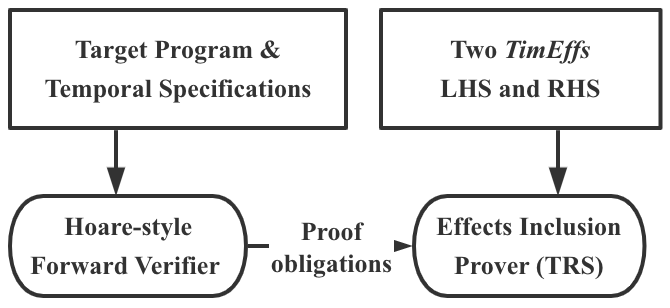
\includegraphics[width=1\columnwidth]{verification.png}
%        \vspace{-3mm}
%\caption{\label{fig:Verification_oberview}System Overview.}
%      \vspace{-1mm}
\caption{\label{fig:Verification_oberview}System Overview.}
\end{wrapfigure}

An overview of our automated verification system is given 
in \figref{fig:Verification_oberview} 
Rounded boxes are the main procedures, and both return \emph{true} 
when the forward reasoning/proving succeeds, return \emph{false} 
otherwise. Rectangular boxes describe the inputs to the procedures.
The input of the TRS is a pair of effects LHS and RHS, referring to the 
inclusion LHS \code{\CONTAIN} RHS to be checked 
\textit{(LHS refers to left-hand-side effects, and RHS refers to right-hand-side 
effects)}. 
Besides, the verifier calls the TRS to prove produced inclusions (dash line). 
The TRS will be explained in \secref{sec:Entailment_Prover}. 



\newcommand{\s}[1]{\code{\{ #1\}}}





 

\subsection{Forward Inference Rules}
\label{Forward_Rules}



 We here present the forward verification rules, 
which are used to systematically accumulate the effects based on 
the syntax of each statement.
\code{\mathcal{P}} denotes the program being checked. 
The rules are in the Hoare-style triples: 
\code{\ \vdash \s{ \Pi, \Theta } \ e\ 
\s{\Pi^\prime, \Theta^\prime}},  where 
$e$ is the given statement;
\s{ \Pi, \Theta } refers to a set of program states. 
The meaning of the transition rules, can be described as: 




\vspace{2mm}
\qquad \code{\s{ \Pi^\prime, \Theta^\prime } = 
\wbigcup_{i{=}0}^{|\s{ \Pi, \Theta }| \text{-} 1}  
\s{\pi_i^\prime, \es_i^\prime}  \ \ where\ \ \code{
  \s{\pi_i, \es_i} {\in} \s{ \Pi^\prime, \Theta^\prime }
}  \ \m{and} \ 
 \vdash  \s{\pi_i, \es_i} \ e \ \s{\pi_i^\prime, \es_i^\prime}.} 
\footnote{\code{|\s{ \Pi, \Theta }|} is the 
size of \code{\s{ \Pi, \Theta }}.}
\vspace{3mm}


\begin{comment}
  

where 
\code{\Theta} is the current effects, 
\code{\Pi} is the current guard, 
%\code{\env} is the current valuation of the variables;
and \s{\Pi_1, \Theta_1}  
is the resulting state by executing \code{e}. 
The program state is initialized using \s{\epsilon, True}. 
These rules transfer program states and systematically accumulate the effects syntactically. 

To define the model, we introduce a stack \env\ and describe 
a program state in a four-elements tuple \s{H, G}, with the following concrete domains:
\begin{flalign*}
G {\defeq} \pi, \qquad\qquad
H  {\defeq} \Theta, \qquad\qquad
\env {\defeq} \code{var {\rightarrow} val }
\end{flalign*}

Let \code{\Pi} represents the pure constraints for all the terms; \code{H} represents the trace of \emph{history}; \code{C} represents the \emph{current} event or a waiting signal; 
\code{T} is a term binding \code{C}; 
\env\ be the environment containing all the local and output signals; 



\end{comment}

\vspace{1mm}
$[FV\text{-}\m{Value}]$  obtains the next program state by 
inheriting the current program state.
$[FV\text{-}Guard]$ computes the effects of \code{e} after concatenating
\code{(b{=}True)}? in to the current program states.  

{{\small\begin{gather*}
  \code{\frac{
  }
{  \vdash \{  \Pi, \Theta \}\  v \ 
\{ \Pi, \Theta \}} \  
 {[FV\text{-}Value]}} 
 \qquad
 \code{\frac{
  \vdash \{  \Pi, \Theta \cdot (b{=}True)? \}\  e \ 
  \{ \Pi^\prime, \Theta^\prime \}
  }
{  \vdash \{  \Pi, \Theta \}\  [b]\ e \ 
\{  \Pi^\prime, \Theta^\prime \}} \  
 {[FV\text{-}Guard]}} 
\end{gather*}}}

\vspace{1mm}
$[FV\text{-}Seq]$ computes  \code{ \{  \Pi_1, \Theta_1\} } 
from \code{e_1}, 
then further gets  \code{ \{  \Pi_2, \Theta_2 \} } by 
continuously computing the behaviors of \code{e_2}, to be the final state.
$[FV\text{-}Par]$ computes behaviors for  \code{e_1} and \code{e_2} independently,
then parallel merges the effects from these two branches.  

{{\small\begin{gather*}
  \code{\frac{ 
 \vdash \{ \Pi, \Theta\}  e_1  \{  \Pi_1, \Theta_1\} 
\ \  \ 
\vdash \{ \Pi_1, \Theta_1\}  e_2   \{  \Pi_2, \Theta_2 \} 
}{
  \vdash \{  \Pi, \Theta \}\  
  e_1;e_2 \ \{ \Pi_2, \Theta_2
  \}} 
   {[FV\text{-}Seq]}}  
\quad 
  \code{\frac{
 \vdash \{ \Pi, \Theta \}  e_1   \{  \Pi_1, \Theta_1\} 
\ \  \ 
\vdash \{  \Pi, \Theta \}  e_2   \{  \Pi_2, \Theta_2 \} 
    }{
\vdash \{   \Pi, \Theta \}\  e_1 || e_2 \ \{ 
\Pi_1  \wedge \Pi_2 , \Theta_1 || \Theta_2
\}}  
{[FV\text{-}Par]}} 
\end{gather*}}}



The \code{[FV\text{-}If\text{-}Else]} computes an 
over-approximation of the program states, by adding different constraints into 
different branches. \code{\Pi \wedge v} enforces 
\code{v} into the pure constraints of every trace in the state, same 
for \code{\Pi \wedge \neg v }.

{{\small\begin{gather*}
  \code{\frac{ 
    \begin{matrix}
\vdash \{ \Pi \wedge v, \Theta    \} \ e_1 \ \{  \Pi_1, \Theta_2 \} 
\qquad 
\vdash \{ \Pi \wedge \neg v , \Theta  \} \ e_2 \ 
\{  \Pi_2, \Theta_2 \}  
\qquad (v\ is\ local)
\end{matrix}}
  {\vdash \s{ \Pi, \Theta}\  \textbf{if}\ v\ \textbf{then}\ e_1\ 
  \textbf{else}\ e_2 \ \s{ \Pi_1, \Theta_2} \cup \s{\Pi_2, \Theta_2} } \  
  {[FV\text{-}If\text{-}Else\text{-}Local]}} 
  \end{gather*}}}
  %\\
%\code{\frac{ 
%  \begin{matrix}
%\vdash \{ \Pi, \Theta    \} \ e_1 \ \{ \Pi_1, \Theta_2 \} 
%\qquad 
%\vdash \{ \Pi , \Theta  \} \ e_2 \ 
%\{  \Pi_2, \Theta_2 \}  
%\qquad (v\ is\ global)
%\end{matrix}}
%{\vdash \s{ \Pi, \Theta}\  \textbf{if}\ v\ \textbf{then}\ e_1\ 
%\textbf{else}\ e_2 \ \s{\Pi, v. \Theta_1 \vee \Theta_2 }} \  
%{[FV\text{-}If\text{-}Else\text{-}Global]}} 



Rule \code{[FV\text{-}Event]} simply constructs a new event and 
concatenates it to the current program states. 
Rule \code{[FV\text{-}Delay]} creates a trace \code{\epsilon\mysharp t}
, where \code{t} is fresh, and concatenates it to the current program states, 
together with the additional constraint \code{t{=}d}. 

  {{\small\begin{gather*}
  \code{\frac{
    \Theta^\prime {=} \Theta\cdot \anyevent{A}(v, \alpha^*) 
    }
  {\vdash \s{ \Pi, \Theta} \  
  \textbf{event} [\anyevent{A}(v, \alpha^*)] 
   \ \{\Pi, \Theta^\prime \}} \   {[FV\text{-}Event]}} 
   \qquad
  \code{\frac{
    \Theta^\prime {=} \Theta\cdot \epsilon\mysharp t \quad (t\ is\ fresh) 
    }
  {\vdash \s{ \Pi, \Theta} \  
  \textbf{delay} [d] 
   \ \{ \Pi \wedge  t {=}d,  \Theta^\prime \}} \   {[FV\text{-}Delay]}} 
\end{gather*}}}



Rule \code{[FV\text{-}Timeout]} computes the effects from \code{e_1} and \code{e_2}
using the starting state \code{\s{\Pi, \epsilon}}. The final states are the union 
of these effects with their corresponding time variables and arithmetic constraints. 
Note that, \code{hd(\Theta_1)} and \code{tl(\Theta_1)} return the head and the tail of 
\code{\Theta_1} respectively. 

{{\small\begin{gather*}
  \code{\frac{
    \begin{matrix}
      \vdash \{\Pi, \epsilon \}\ e_1 \ \{  \Pi_1, \Theta_1\} 
      \qquad 
      \vdash \{ \Pi, \epsilon \}\ e_2 \ \{  \Pi_2, \Theta_2 \} 
      \\
      \s{\Pi_f, \Theta_f} {=} \s{\Pi_1  \wedge t_1{\leq}d, (hd(\Theta_1)\mysharp t \cdot tl(\Theta_1))}
      \cup 
  \s{\Pi_2  \wedge t_2{>}d,  (\Theta_2\mysharp t)}   
  \quad (t_1, t_2\ are\ fresh)     
\end{matrix}
  }
  {\vdash \s{ \Pi, \Theta} \  
  e_1\ \textbf{timeout} [d] \  e_2
   \ \s{\Pi_f, \Theta \cdot \Theta_f} } \   {[FV\text{-}Timeout]}} 
\end{gather*}}}


Similar to \code{[FV\text{-}Timeout]}, \code{[FV\text{-}Ddl]} computes the effects 
from \code{e} and adds an upper time-bound to the result. 

{{\small\begin{gather*}
  \code{\frac{
    \begin{matrix}
      \vdash \{ \Pi, \epsilon\}\ e \ \{  \Pi_1, \Theta_1\} 
  \quad (t\ is\ fresh)     
\end{matrix}
  }
  {\vdash \s{ \Pi, \Theta} \  
  \textbf{deadline}  [d] \ e 
   \ \s{\Pi_1  \wedge t{\leq}d, \Theta  \cdot (\Theta_1\mysharp t)} }   
    {[FV\text{-}Ddl]}} 
  \end{gather*}}}


  Rule \code{[FV\text{-}Meth]} initializes the current effects state 
using the declared precondition, accumulates the effects from the method body, 
to obtain \code{ \s{\Pi, \Theta}}; then  it
checks the  inclusion between \code{ \s{\Pi, \Theta}} and the concatenation of 
the precondition and the postcondition\footnote{Here, 
\code{\effect_{post}} only needs to capture the effects from the current method body, excluding the history effects specified in \code{\effect_{pre}}. }.
  
{{\small\begin{gather*}
\code{\frac{  \vdash \s{\effect_{pre}}
 \ e \  \{ \Pi, \Theta \} \qquad   \{ \Pi, \Theta \} \CONTAIN  
 \effect_{pre} \cdot \effect_{post}}{  \vdash  \ mn  \ {x^*}\ \{\textbf{req}\ \effect_{pre}\ 
  \textbf{ens}\  \effect_{post}\} \ \{ e \}}   {[FV\text{-}Meth]}}  
  \end{gather*}}}



Rule \code{[FV\text{-}Call]} first checks whether the instantiated 
  precondition of callee, \code{[v^*/x^*]\effect_{pre}}, is satisfied by 
  the current program state. When the check is succeeded, the final states are 
  formed by concatenating the  
  instantiated postcondition to the current states. 

  %, in which we use an auxiliary function \code{rev} to reverse the event sequences of effects.
{{\small\begin{gather*}
\code{\frac{
\begin{matrix}
{\code{  mn  \ {x^*}\ \{\textbf{req}\ \effect_{pre}\ \textbf{ens}\  \effect_{post}\} \ \{ e \} \in \mathcal{P}\ \ }}
\\
\text{\code{ \s{ \Pi, \Theta} \CONTAIN [v^*/x^*] \effect_{pre}   
\qquad   \effect_f =  \s{ \Pi, \Theta} \cdot  [v^*/x^*]\effect_{post}}}
\end{matrix}}
{\vdash \s{ \Pi, \Theta} \ mn({v^*})  \ 
\effect_f} \ {[FV\text{-}Call]}}
\end{gather*}}}


\begin{theorem}[Soundness of the Forward Rules]\label{Soundness_forward_rules}
  Given any system configuration \code{\zeta = (\env, e)}, by applying the operational
  semantics rules, 
  if \code{(\env, e) {\rightarrow^*} (\env^\prime, ())} produces concrete 
  execution time \code{d} and event sequence \code{\varphi}, and the forward verifier reasons \code{ \vdash  
  \s{\env, \epsilon} \ e\  \s{\Pi, \Theta}}, then, \\
  \code{\qquad \qquad \qquad \qquad  \qquad 
   \exists (\pi\wedge \es) \in \s{\Pi, \Theta} } such that 
  \code{d, \env^\prime, \varphi  \models (\pi\wedge \es)}. 
  %. 

%  pair $(\env , e)$ where $\env$ is a variable valuation function and $e$ is an expression.
  \end{theorem}
  
  
  \begin{proof}
   % By induction.        
    See \appref{proof:SoundnessProof_FE}.
  \end{proof}


\section{Temporal Verification via a TRS}
\label{sec:Entailment_Prover}


The TRS  is an automated entailment checker to prove language 
inclusions between \timedEffects, cf. \defref{Inclusion} and 
\tabref{tab:rewriting_tree_send} It is triggered i) prior to 
temporal property assertions; ii) prior to function calls for the 
precondition checking; and iii) at the end of verifying a function 
for the post condition checking. Given two effects 
\code{\effect_1} and \code{\effect_2}, the TRS decides if the inclusion \code{\effect_1 \CONTAIN  \effect_2 } is valid. 

During the effects rewriting process, the inclusions are in the form of \code{\Gamma \vdash  \effect_1 \CONTAIN^{\effect}  \effect_2 }, a shorthand for: \code{\Gamma \vdash  \effect \cdot \effect_1 \CONTAIN   \effect \cdot  \effect_2}. To prove such inclusions is to check whether all the possible timed traces in the antecedent \code{\effect_1} are legitimately allowed  in the possible timed traces from the consequent \code{\effect_2}.
\code{\Gamma} is the proof context, i.e., a set of effects inclusion hypothesis, \code{\effect} is the history effects from the antecedent that have been used to match the effects from the consequent.
Note that \code{\Gamma}, \code{\effect} are derived during the inclusion proof. 
The inclusion checking is initially invoked with \code{\Gamma{=}\{\}} and 
\code{\effect{=} True \wedge  \epsilon}. 







\paragraph{\textbf{Effects Disjunctions.}}
An inclusion with a disjunctive antecedent succeeds if both disjunctions entail the consequent.  An inclusion with a disjunctive consequent succeeds if the antecedent entails either of the disjunctions.  
{ 
 \begin{gather*}
\frac{ \begin{matrix}
    \text{\code{\Gamma \vdash  \effect_1 \CONTAIN  \effect  \qquad \Gamma \vdash \effect_2 \CONTAIN  \effect}}
  \end{matrix}}{\Gamma \vdash  \effect_1 \vee \effect_2 \CONTAIN  \effect}\  \code{[LHS\text{-}OR]}
\qquad
\frac{ \begin{matrix}
    \text{\code{\Gamma \vdash  \effect \CONTAIN  \effect_1  \quad or \quad \Gamma \vdash \effect \CONTAIN  \effect_2}}
  \end{matrix}}{\Gamma \vdash    \effect \CONTAIN \effect_1 \vee \effect_2}\  \code{[RHS\text{-}OR]}
\end{gather*}



}

\vspace{2mm}
Now, the inclusions are disjunction-free formulas. 
Next we provide the definitions and the key implementations\footnote{As 
the implementations according to basic regular expressions can be found 
in prior work \cite{DBLP:conf/fsttcs/KeilT14}. 
%Here, we focus on presenting 
%the definitions and how do we deal with dependent values in the effects, 
%as the key novelties of this work. 
%More detail implementations can be found in the extended technical report\citeref{Demo}.
} of Nullable, First and Derivative respectively. Intuitively, 
the Nullable function \code{\delta_{{\pi}}(\es)} returns a Boolean 
value indicating whether \code{{\pi} \wedge \es} contains the empty 
trace; the First function \code{fst_{{\pi}}( \es)} computes a set of 
 initial \emph{heads}, denoted as \code{h},  of \code{{\pi} \wedge \es}; and the Derivative 
function \code{D^{\pi}_{h}(\es)} computes a next-state 
effects after eliminating the head  \code{h} from the current 
effects \code{{\pi} \wedge \es}. 

%\subsection{closure of clock constraints}
%how to eliminate the unobservable transitions. 
%
%we allow the $ \epsilon$transitions without carrying constraints and resetting clocks at the same time. 


\begin{definition}[Nullable \footnote{The proof obligations are 
  discharged using the Z3 SMT prover, while deciding the nullability of effects constructed by symbolic terms, represented by \code{SAT({\pi})}.}]\label{Nullable}
Given any \code{\effect {=} \pi  \wedge  \es}, %we define 
%\code{\delta_{{\pi}}(\es)} to be \\
{
  \code{\delta_{{\pi}}(\es) :bool {=}
  \begin{cases}
        \code{true} & \code{if\  \epsilon \in \llbracket {\pi}  \wedge  \es \rrbracket}\\
        \code{false} & \code{if\  \epsilon \notin \llbracket {\pi}  \wedge  \es \rrbracket}
      \end{cases} }
      }, where:  
\begin{comment}
 a boolean value, indicating whether \code{\effect} contains the empty trace, i.e., $\epsilon$. 
We define recursively:  
\end{comment} 
{ 
\begin{gather*}
\code{\delta_{\pi}(\bot ) {=} false} 
\qquad\quad
\code{\delta_{\pi}( \epsilon) {=} true} 
\qquad\quad
\code{\delta_{\pi}(\ev){=} false}   
\qquad\quad
\code{\delta_{\pi}(\pi^\prime?){=} false}  
\qquad\quad\
    \code{\delta({\es^\star} ) {=} true}   
\\ 
\ \ 
\code{\delta_{\pi}(\es \cdot \es_2) {=} \delta(\es_1) \wedge \delta(\es_2)}
\qquad\qquad\quad
  \code{\delta_{\pi}(\es_1 \vee \es_2) {=} \delta(\es_1) \vee \delta(\es_2)}   
  \\
\code{\delta_{\pi}(\es_1 || \es_2) {=} \delta(\es_1) \wedge \delta(\es_2)}
\qquad\qquad\quad
 \code{\delta_{\pi}(\es \mysharp  t) {=} SAT ({\pi} \wedge (t {=} 0) )}
\end{gather*}}
\end{definition}


%Next, we define the novel  \emph{First} function used in this work, denoted using \code{fst}. 
%but helps to build up our \emph{First} function \code{fst}. 


\vspace{2mm}
\begin{definition}[Heads]\label{Heads}
If \code{h} is a head of \code{\pi \wedge \es}, then there exist 
\code{\pi^\prime} and \code{\es^\prime}, 
such that \code{\pi \wedge \es} {=} \code{\pi^\prime \wedge h \cdot \es^\prime}. 
   %We adopt the following naming convention for transition labels: 
A head can be  $t$, denoting a pure time passing; 
  $\ev $, denoting an instant event passing; or 
  $(\ev, t)$, denoting an event passing which takes time \code{t}. 
\end{definition}


\vspace{2mm}
\begin{definition}[First]\label{First}
  Given any \code{\effect {=} \pi \wedge \es},
  \code{fst_{{\pi}}(\es)} returns a set of heads, be the set of initial elements   
  derivable from effects \code{\pi \wedge \es}, where: 
    { 
   \begin{gather*} 
  \code{fst_{{\pi}}( \bot ) {=} \{\} } \qquad\quad 
  \code{fst_{{\pi}}( \epsilon) {=}  \{\} } \qquad\quad
  \code{fst_{{\pi}}( \ev) {=} \{ \ev \}  }
  \qquad\quad
  \code{fst_{{\pi}}(  \epsilon \mysharp  t) {=}  \{ t \}}
  \qquad\quad
  \code{fst_{{\pi}}( {\es^\star} ) {=} fst_{{\pi}}({ \es})}
   \\
   \code{fst_{{\pi}}(\es \mysharp  t) {=}  \{(\ev, t^\prime) \ | \ \ev \in fst_{\pi}(\es) \}} 
   \ \ \  \emph{($t^\prime$\ is\ fresh)}
  \quad  
  \qquad
  \code{fst_{{\pi}}(  \es_1 {\vee} \es_2) {=} fst_{{\pi}}(  \es_1) \cup fst_{{\pi}}(  \es_2)  }  
  \\
  \code{fst_{{\pi}}( \pi^\prime? ) {=} \{\tau(\pi^\prime); \tau(\neg \pi^\prime)\}  }
      \qquad\qquad\qquad 
     \code{fst_{{\pi}}(  \es_1 {||} \es_2) {=} fst_{{\pi}}(  \es_1) \cup fst_{{\pi}}(  \es_2)  }   
     \\
  {
  \code{fst_{{\pi}}(\es_1 \cdot \es_2) {=} } 
  \begin{cases}
        \code{\code{fst_{{\pi}}(  \es_1)} \cup \code{fst_{{\pi}}(  \es_2)} } \quad   & \code{ if\ \  \delta(\es_1) {=} true}\\
        \code{\code{fst_{{\pi}}(  \es_1)}} & \code{  if\ \  \delta(\es_1) {=} false}
      \end{cases} 
      }  
  \end{gather*}
  }
\end{definition}

\begin{comment}
  \begin{definition}[Heads Subsumption]\label{Subsumption1}
Given two time instances \code{(I, \pi_1, t_1)} and \code{(J, \pi_2, t_2)}, we define the subset relation \code{(I, \pi_1, t_1) {\subseteq} (J, \pi_2, t_2)} as:  \code{I {\subseteq} J} and \code{\pi_1[t_2/t_1]  {\Rightarrow}   \pi_2  }.

\end{definition}
\end{comment}


\vspace{2mm}
\begin{definition}[Partial Derivative]\label{Derivative}
  Given any \code{\effect {=}\pi \wedge  \es}, 
  %and a variable valuation function \code{\env}, 
  the partial derivative \code{D^{\pi}_{h}( \es)} 
   computes the  effects for the 
  left quotient \code{(h)^{\text{-}1}\llbracket \pi \wedge \es 
  \rrbracket}\footnote{Intuitively, the partial derivative refers to the left quotient of a language equation, for example, for REs, \code{x^{{-}1} \llbracket x\cdot y\rrbracket {=} y};  \code{y^{{-}1} \llbracket x\cdot y\rrbracket {=} \bot }; and  \code{y^{{-}1} \llbracket x + y\rrbracket {=} \epsilon}. Here we come up with a new notion of partial derivative for \timedEffects. 
  }. 

  \begin{gather*}
  \code{D^{\pi}_{h}( \bot ) {=}}  \code{False \wedge \bot } 
  \qquad\qquad 
  \code{D^{\pi}_{h}(   \epsilon) {=}}  \code{False \wedge \bot } 
  \qquad\qquad
  \code{D^{\pi}_{h}(  \ev^\prime) } {=} 
  \code{  (\pi \wedge h{=}\ev^\prime) \wedge \epsilon} 
  \\
  {
   \code{\code{D^{\pi}_{h}( \pi^\prime?)} {=}}
  \begin{cases}
        \code{\pi \wedge \pi^\prime? } &\code{if\ h \not\Rightarrow  \pi^\prime}   \\
        \code{\pi \wedge \epsilon} & \code{if\ h \Rightarrow \pi^\prime} 
      \end{cases} 
      }
      \qquad \quad \ \ \ 
  {
   \code{D^{\pi}_{h}( \es_1  \cdot  \es_2) {=} }
  \begin{cases}
        \code{D^{\pi}_{h}( \es_1) \cdot  \es_2\ \vee \  D^{\pi}_{h}( \es_2)}  &\code{if\ \delta_{\pi}(\es_1) {=} true}   \\
        \code{D^{\pi}_{h}( \es_2) \cdot  \es_2} & \code{if\ \delta_{\pi}(\es_1) {=} false} 
      \end{cases} 
      }
  \\
  \code{D^{\pi}_{h}(  {\es^\star}) } {=} \code{ D^{\pi}_{h}(  {\es}) \cdot {\es^\star}}  
  \qquad\quad \ \ \ 
  \code{D^{\pi}_{h}(  \es_1 {\vee} \es_2) } {=} \code{ D^{\pi}_{h}(  \es_1) \vee D^{\pi}_{h}(  \es_2)} 
  \qquad \quad\ \ \ 
  \code{D^{\pi}_{h}( \es_1 {||}\es_2)} {=} \code{\Bar{\Bar{D}}^{\pi}_{h}( \es_1)} || \code{\Bar{\Bar{D}}^{\pi}_{h}( \es_2)} 
   \\
   \code{D^{\pi}_{\ev}(  \es \mysharp t) } {=} {\bigvee}
   \code{ \{ (\pi^\prime \wedge \es^\prime  \mysharp t) \ | \ (\pi^\prime, \es^\prime) \in D^{\pi}_{\ev}(\es) \} } 
\qquad 
   \code{D^{\pi}_{t}(  \es \mysharp t^\prime) } {=} 
   \code{ (\pi \wedge t{+}t^{\prime\prime}{=}t^\prime) \wedge  
   \es \mysharp t^{\prime\prime} \ \ \  {(t^{\prime\prime}\ is\ fresh)} } 
  \end{gather*}
  \end{definition}
  
Notice that the derivatives of a parallel composition makes use of the \emph{Parallel Derivative} \code{\Bar{\Bar{D}}^{\pi}_{h}(\es)}, defined as follows: 
 
\begin{definition}[Parallel Derivative]\label{Derivative_maybe}
    Given any \code{\effect {=} \pi \wedge \es}, and a variable valuation function \code{\env}, 
    the parallel derivative is defined as: {
      \code{\Bar{\Bar{D}}^{\pi}_{h}( \es) {=}
      \begin{cases}
            \code{ \es} & \code{if\ D^{\pi}_{h}(\pi \wedge \es) = (False \wedge \bot )}\\
            \code{D^{\pi}_{h}( \es)} & \code{otherwise}
          \end{cases} }
    }.
  \end{definition}


  \vspace{2mm}
\subsection{Rewriting Rules}
\label{InferenceRules}
Given the well-defined auxiliary functions above, we now discuss the key steps and related rewriting rules that we may use in such an effects inclusion proof.  


\begin{enumerate}
\item 
\textbf{Axiom rules.}
\label{Base}
Analogous to  the standard propositional logic, \code{\bot } (referring to \textit{false}) entails any effects, while no \textit{non-false} effects entails \code{\bot }.
 \begin{gather*}
  \codeme{\frac{
\begin{matrix}
\end{matrix}
}{\text{\code{ \Gamma  \vdash \pi : \bott   \CONTAIN \effect }}}\ [Bot\text{-}LHS]}
\qquad\qquad\quad
\codeme{\frac{
\begin{matrix}
\effect \neq  \pi : \bott 
\end{matrix}
}{\text{\code{\Gamma  \vdash  \effect \not\CONTAIN  \pi : \bott }}} \ \codeme{  [Bot\text{-}RHS]} }
\end{gather*}

\item 
\textbf{Disprove (Heuristic Refutation).}
\label{Refutation}
This rule is used to disprove the inclusions when the antecedent is nullable, while the consequent is not nullable. Intuitively, the antecedent contains at least one more trace (the empty trace) than the consequent. Therefore, the inclusion is invalid. 
 \begin{gather*}
\frac{
\begin{matrix}
\text{\codeme{\delta(\es_1) \wedge \neg \delta(\es_2) }}
\end{matrix}
}{\text{\code{\Gamma  \vdash  \pi_1 : \es_1 \not\CONTAIN  \pi_2 : \es_2 }}}\ \codeme{  [DISPROVE]} 
\qquad\ \ 
\frac{
\begin{matrix}
\text{\code{\pi_1 \Rightarrow \pi_2 \quad\ \  
\m{fst}_{\pi_1}(\es_1) = \{\}
%\es_1 \subseteq \es_2 
}}
\end{matrix}
}{\text{\code{\Gamma   \vdash  \pi_1 : \es_1 \CONTAIN  \pi_2 : \es_2 }}}\ \codeme{  [PROVE]} 
\end{gather*}

\item 
\textbf{Prove.}
\label{Prove}
We use two rules to prove an inclusion: (i) $\codeme{[PROVE]}$ is 
used when the fst set of the antecedent is empty; and 
(ii) $\codeme{[REOCCUR]}$ to prove an inclusion
when there exist inclusion hypotheses 
in the proof context $\m{\Gamma}$, which are able to 
soundly prove the current goal. One of the special cases of 
this rule is when the identical inclusion is shown in the proof 
context, we then terminate the procedure and prove it as a valid 
inclusion. 
 \begin{gather*}
\frac{
\begin{matrix}
\text{\codeme{ (\pi_1 : \es_1 \CONTAIN \pi_3 : \es_3) \in \Gamma  }} 
\quad\ \ 
\text{\codeme{(\pi_3 : \es_3 \CONTAIN  \pi_4 : \es_4) \in {\Gamma} }} \quad\  \ 
\text{\codeme{ (\pi_4 : \es_4 \CONTAIN \pi_2 : \es_2) \in {\Gamma}  }}
\end{matrix}
}{\text{\code{\Gamma  \vdash  \pi_1 : \es_1 \CONTAIN  \pi_2 : \es_2 }} }
\ \codeme{[REOCCUR]}
\end{gather*}

\item 
\textbf{Unfolding (Induction).}
\label{unfolding}
This is the inductive step of unfolding the inclusions. Firstly, 
we make use of the auxiliary function \code{fst} to get a set of 
heads \code{H}, which are all the possible initial time instances 
from the antecedent. 
Secondly, we obtain a new proof context \code{\Gamma^\prime} by 
adding the current inclusion, as an inductive hypothesis, into 
the current proof context \code{\Gamma}. 
Thirdly, we iterate each element \code{h \in H}, and compute the 
partial derivatives (\emph{next-state} effects) of both the 
antecedent and consequent w.r.t \code{h}. The proof 
of the original inclusion succeeds if all the derivative 
inclusions succeed.
\begin{gather*}
\frac{ \begin{matrix}
\text{\codeme{F = \m{fst}_{\pure{\pi_1}}(\es_1)\qquad\qquad \Gamma^\prime = \Gamma,  (
\pure{\pi_1} : \es_1 \CONTAIN \pure{\pi_2} : \es_2
)} }\\
    \text{\codeme{\forall (I, \pi, t)\in F. \   (\Gamma^\prime  \vdash \   D_{(I, \pi, t)}^{\pure{\pi_1}}( \es_1) \CONTAIN    D_{(I, \pi, t)}^{\pure{\pi_2}}( \es_2) )}}
  \end{matrix}}
   { \text{\codeme{  \Gamma  \vdash \pure{\pi_1} : \es_1 \CONTAIN \pure{\pi_2} : \es_2 }}}\  \codeme{[UNFOLD]} 
\end{gather*}


\item 
\textbf{Normalization.}
We present some normalization rules to soundly transfer the timed effects into a normal form, in particular after getting their derivatives. 
Before getting into the above inference rules, we assume that the effects formulae are tailored accordingly based on the axioms shown in
\tabref{table:normalization}
We built the axiom system on top of an axiom system \code{F_1}, from (A1) to (A10), suggested by \cite{DBLP:journals/jacm/Salomaa66}, 
which was designed for regular languages. We develop axioms (A11) 
to (A16) to further accommodate effects constructed by 
\code{||} and \code{\mysharp}.


\begin{table}[ht]
  \caption{Some Normalization Axioms for \timedEffects.}
  \label{table:normalization}
  \setlength{\tabcolsep}{10pt}
  \renewcommand{\arraystretch}{1.2}
  \centering
  \begin{tabular}{rl}
  \footnotesize
  
  \begin{minipage}[t]{0.36\textwidth}
  \begin{tabular}{||l|l}
  \hline
  (A1)  &
  \code{\es_1 \vee (\es_2 \vee \es_3) \rightarrow   (\es_1 \vee \es_2) \vee \es_3 }\\
  \hline
  (A2)  &
  \code{\es_1 \cdot (\es_2 \cdot \es_3)\rightarrow     (\es_1 \cdot \es_2) \cdot \es_3 }\\
  \hline
  (A3)  &
  \code{\es \cdot (\es_1 \vee \es_2)  \rightarrow \es \cdot \es_1  \vee \es \cdot \es_2 }\\
  \hline
  (A4)  &
   \code{(\es_1 \vee \es_2)\cdot \es   \rightarrow \es_1 \cdot \es   \vee  \es_2 \cdot \es}\\
  \hline
  (A5)  &
   \code{\es \vee \es   \rightarrow \es}\\
  \hline
  (A6)  &
   \code{  \es \cdot \epsilon   \rightarrow \es}\\
  \hline
  (A7)  &
   \code{  \es \cdot  \bot \rightarrow \bot}\\
  \hline
  (A8)  &
  \code{\es \vee \bot   \rightarrow \es}\\
  \hline


  
  
  
  \end{tabular}
    \end{minipage} 
   
    &
  \footnotesize
    \begin{minipage}[t]{0.6\textwidth}
  \begin{tabular}{||l|l|}
  \hline
  (A9)  &
  \code{\epsilon \vee (\es \cdot \es^\star)   \rightarrow  \es^\star}\\
  \hline
  (A10)  &
  \code{(\epsilon \vee \es)^\star   \rightarrow  \es^\star}\\
  \hline
  (A11)\code{^\heartsuit}  &
  \code{ \es\ ||\  \epsilon \rightarrow \es}\\
  \hline
  (A12)\code{^\heartsuit}  &
  \code{ \es\ ||\ \bot  \rightarrow \bot }\\
  \hline
  (A13)\code{^\heartsuit}  &
  \code{\bot \mysharp  t \rightarrow  \bot }\\
  \hline
  (A14)\code{^\heartsuit}  &
  \code{\pi \wedge (\es \mysharp  t_1 ) \mysharp  t_2 
  \rightarrow \pi  \wedge (t_1 {=} t_2) \wedge \es \mysharp  t_1 }\\
  \hline
  (A15)\code{^\heartsuit}  &
   \code{(\epsilon \mysharp  t_1) ||(\epsilon \mysharp  t_2) \rightarrow 
   (t_1 {\geq}t_2 \wedge\epsilon\mysharp t_1) \vee   (t_1 {<}t_2 \wedge \epsilon\mysharp t_2) }\\
  \hline
  (A16)\code{^\heartsuit}  &
   \code{{{False}} \wedge \es = {\pi} \wedge \bot  \rightarrow {{False}} \wedge \bot }\\
  \hline

  
  
  \end{tabular}
    \end{minipage}
    
  
   
  \end{tabular}
  \vspace{-2mm}

  \end{table}
  
  
  
\end{enumerate}






 
\begin{theorem}[Termination  of the TRS]\label{termination}
The rewriting system TRS is terminating.
\end{theorem}
\begin{proof}
See %the technical report\cite{TR}. 
\appref{proof:TerminationProof}.
\end{proof}

 \begin{theorem}[Soundness of the TRS]\label{Cyclicsoundness}
Given an inclusion \code{\effect_1 \CONTAIN \effect_2}, if the TRS returns \code{TRUE} when proving \code{\effect_1 \CONTAIN \effect_2}, i.e., it has a cyclic proof, 
then \code{\effect_1 \CONTAIN \effect_2} is valid.
\end{theorem}


\begin{proof}
See %the technical report\cite{TR}. 
\appref{proof:SoundnessProof}.
\end{proof}





\section{Implementation and Case Study}
\label{sec:Evaluation}


To show the feasibility of our approach, we have prototyped 
our automated verification system 
using OCaml. The proof obligations generated by the verifier 
are discharged using constraint solver Z3 
\citep{DBLP:conf/tacas/MouraB08}. 
We prove termination and soundness of the TRS. We validate 
the front-end forward verifier against the state-of-the-art PAT 
\cite{DBLP:conf/cav/SunLDP09} model checker for conformance. 
Next, we show experimental results and case studies to evaluate our proposals. 

\subsection{Experimental Results}
\label{subsec:Experimental_Results}


%We claim that the extra expressiveness gained from our logic is the symbolic time-bounds. The timed effects represent not only one exact Timed Automata but also a set of Timed Automata. Together with our back-end inclusion solver, it enables a verification framework for a group of Automata. More specifically, instead of running the model checker many times for one non-deterministic time-bound at each time, we can define arithmetic constraints bounding the time variable. And to test that, we cover a number of test cases with function calls, and the callee's parameters would be used as the time bounds.






\begin{table}[!ht]
\caption{\label{tab:Experimental} Experimental Results. }
\vspace{-2mm}
\centering
\renewcommand{\arraystretch}{1}
\begin{tabular} {c|c|c|c|c |c|c|c}
\hline
\textbf{No.} & \textbf{LOC} & \textbf{Infer(ms)} & \textbf{$\mysharp$Prop(\cmark)}   
& \textbf{Avg\text{-}Prove(ms)} & \textbf{$\mysharp$Prop(\xmark)}   & \textbf{Avg\text{-}Dis(ms)} &\textbf{$\mysharp$AskZ3} \\ \hline\hline
1    &    30    & 0.031  &  5     &  4.185   & 5   &  3.242  & 68 \\ \hline
2    &    35    & 0.038  &  3     &  13.761  & 7   &  9.331  & 214 \\ \hline
3    &    44    & 0.049  &  4     &  12.149  & 6   & 7.853   & 215 \\ \hline
4    &    72    & 0.061  &  5     &  37.268 & 5   & 28.3054 & 617 \\ \hline
5    &    95    & 0.105  &  7     &  6.139    & 7   &  5.238  & 186 \\ \hline
6    &    108   & 0.16   &  7     &  43.667    & 7   &  17.178  & 818 \\ \hline
7    &    106   & 0.142  &  7     &  18.776    & 7   &  8.432  & 346 \\ \hline
8    &    144   & 0.141  &  7     &  22.238    & 7   &  10.051  & 426 \\ \hline
9    &    155   & 0.308  &  9     &  194.666   & 9   &  56.344  & 4059 \\ \hline
10   &    174   & 0.373  &  9     &  78.132   & 9   &   24.665  & 1740 \\ \hline
11   &    196   & 0.557  &  9     &  111.100   & 9   &   31.262  & 2403 \\ \hline
12   &    213   & 0.516  &  9     &  114.667   & 9   &  30.284   & 2484 \\ \hline
13   &    265   & 1.895  &  11    & 616.619    & 11  &  302.975  & 9068 \\ \hline
14   &    271   & 1.702  &  11    &  302.145   & 11  &  131.938  & 7779 \\ \hline     
15   &    276   & 2.121 & 11     &  466.174  & 11  &   181.116  & 12239 \\ \hline
16   &    314   & 1.654 &  11    & 1094.231   & 11  &  465.704  & 32620 \\ \hline            
%\hline
%\textbf{\quad \ \ Total}  & 2546    &  235   &  446.88   &   305.33   \\ \hline
\end{tabular}
%  \vspace{-1mm}
\end{table}

\autoref{tab:Experimental} presents the evaluation results of a microbenchmark. % summary of a lightweight . 
In this experiment, we select 16 \timedL\ programs, and  annotate temporal specifications
with a roughly 1:1 ratio for succeeded/failed cases. 
Times are counted using milliseconds, and the experiment is done on 
a MacBook Pro with a 2.6 GHz 6-Core Intel Core i7 processor. 
The table records: 
\textbf{No.}, the index of the program;
\textbf{LOC}, lines of code; 
\textbf{Infer(ms)}, effects inference time; 
\textbf{$\mysharp$Prop(\cmark)}, number of valid properties; 
\textbf{Avg\text{-}Prove(ms)}, average proving time for the valid properties;
\textbf{$\mysharp$Prop(\xmark)}, number of invalid properties; 
\textbf{Avg\text{-}Dis(ms)}, average disproving time for the invalid properties; and 
\textbf{$\mysharp$AskZ3}, number of querying Z3 solver through out the experiments.


\paragraph{Discussion:} Generally, the inference time and proving 
time increase while the program's length increases. 
Besides, while \emph{the number of querying Z3 per property} (\textbf{$\mysharp$AskZ3}/(\textbf{$\mysharp$Prop(\cmark)} +\textbf{$\mysharp$Prop(\xmark)})) 
goes up, the 
proving/disproving time goes up.
Furthermore, we notice that 
%that no matter how long the programs are, 
the disproving
times for invalid properties are constantly lower than the proving process, 
regardless of the program complexity. This finding echos the 
insights from prior TRS-based works \cite{DBLP:conf/icfem/SongC20,DBLP:journals/tcs/AntimirovM95,DBLP:journals/ijfcs/AlmeidaMR09,DBLP:conf/fsttcs/KeilT14,DBLP:journals/jcss/Hovland12}, 
which suggest that TRS is a better average-case algorithm than 
those based on the comparison of automata.  

As a summary: a TRS is efficient because 
\emph{it only constructs automata as far as it needs}, which makes 
it more efficient when disproving incorrect specifications, as we can 
disprove it earlier without constructing the whole automata. In other 
words, the more incorrect specifications are, the more efficient our solver is.


%
%\subsubsection{Experimental Results}~\\
%\label{subsec:Experimental_Results}
%
%\begin{table}[ht]
%        \vspace{-2mm}
%\caption{\label{tab:Experimental} The experiments are based on 16 real world C programs, we record the lines of code (LOC), the number of testing temporal properties ($\mysharp $Prop.), and the (dis-) proving times (in time units) using PAT and our T.r.s respectively. }
%\centering
%\footnotesize
%\renewcommand{\arraystretch}{1.1}
%\begin{tabular} {l|c|c|c|c}
%\hline
%\textbf{Programs} & \textbf{LOC} & \textbf{$\mysharp $Prop.}  & \textbf{PAT(ms)} & \textbf{T.r.s(ms)} \\ \hline\hline
%1. Chrome\_Dino\_Game    &      80    &    12  &  32.09 &  7.66  \\ \hline
%2. Cradle\_with\_Joystick  &      89     &   12   &  31.22    &   9.85  \\ \hline
%3. Small\_Linear\_Actuator  &    180  &     12  &   21.65      &  38.68  \\ \hline
%4. Large\_Linear\_Actuator &    155   &    12   &  17.41   &   14.66   \\ \hline
%5. Train\_Detect  &                    78   &     12    &   19.50   & 17.35     \\ \hline
%6. Motor\_Control  &                 216  &    15  &     22.89  &  4.71  \\ \hline
%7. Train\_Demo\_2  &                133  &   15    &     49.51   &  59.28   \\ \hline
% 8. Fridge\_Timer  &                  292   &    15   &   17.05   & 9.11 \\ \hline
%  9. Match\_the\_Light   &         143     &    15  &  23.34    &  49.65 \\ \hline
%   10. Tank\_Control  &              104   &    15    &  24.96   &   19.39 \\ 
%     \hline
%  \textbf{\quad \ \ Total}  & 2546    &  235   &  446.88   &   305.33   \\ \hline
%\end{tabular}
%        \vspace{0mm}
%\end{table}
%
%
%        \vspace{-2mm}
%
%
%


\subsection{Case Studies}
\label{subsec:Case_Studies}

%Meanwhile, we further demonstrate the flexibility and expressiveness of our effects logic. 

%how our proposal makes it flexible for different effects logics.     









\subsubsection{Prove it when Reoccur}

   %   \vspace{-2mm}
%(\code{\{Go\} \Rightarrow \_})
%(\code{\{Ready\} \Rightarrow \_}, \code{t_L^2 \Rightarrow true})
Termination of TRS is guaranteed because the set of derivatives 
to be considered is finite, and possible cycles are detected 
using \emph{memorization} \cite{DBLP:conf/tableaux/Brotherston05}, 
i.e., the rule $\codeme{[REOCCUR]}$. 
% Check out this following example: 




{
\begin{table}[ht]
      \vspace{0mm}
\caption{\label{tab:reoccur} The reoccurrence proving example. 
\code{(I)} The main rewriting proof tree; \code{(II)} Right hand side sub-tree of the rewriting process.}
      
\vspace{-1mm}
\begin{adjustbox}{width=1\textwidth}
 \Large\begin{tabular}[t]{l}
  \hline\\
 

\code{(I):}\
{

\begin{prooftree}


\hypo{
  \code{
   % \textcolor {darkred}{True} \Rightarrow  \textcolor {darkred}{True} \qquad
   % \epsilon \CONTAIN \epsilon
   {\textcircled{4}\siderule{\codeme{[PROVE]}}}
  }
}

\infer[dashed]1[]{
  \code{
    \textcolor {darkred}{True} \wedge \epsilon \CONTAIN
    \textcolor {darkred}{True} \wedge \epsilon
  }
}

\infer[dashed]1[{\textcircled{3}\siderule{\codeme{[Normalisation]}}}]{
  \code{
    \textcolor {darkred}{True} \wedge \cancel{  B  } \CONTAIN
    \textcolor {darkred}{True} \wedge \cancel{ \epsilon \cdot   B  }
  }
}

\infer[dashed]1[{\textcircled{2}\siderule{\codeme{[UNFOLD]}}}]{
  \code{
    \textcolor {darkred}{True} \wedge   B   \CONTAIN
    \textcolor {darkred}{t_R{<}4} \wedge   A  ^\star \mysharp  t_R \cdot   B  
  }
}
\hypo{(\code{II})}

\infer[dashed]1[{\siderule{}}]{
  \code{
    \textcolor {darkred}{t_L{<}3}  \wedge    A  ^\star \mysharp  t_L  \cdot    B  
    \CONTAIN
    \textcolor {darkred}{t_R{<}4}  \wedge    A  ^\star \mysharp  t_R  \cdot    B  
  }
}

\infer[dashed]2[{\textcircled{1}\siderule{\codeme{[OR\text{-}LHS]}}}]{
  \code{
    \textcolor {darkred}{t_L{<}3} \wedge   A  ^\star \mysharp  t_L \cdot   B  
    \vee \textcolor {darkred}{True} \wedge   B   \CONTAIN
    \textcolor {darkred}{t_R{<}4} \wedge   A  ^\star \mysharp  t_R \cdot   B  
  }
}
\end{prooftree}}
\\~\\ 

\hline \\
\code{(II):}
{\begin{prooftree}
\hypo{
  \code{
    \textcolor {
      darkred}{t_L{<}3 \wedge } \ \textcolor {
        blue}{t_L^1{+}t_L^2{=}t_L \wedge  t_R{=}t_R^1{+}t_R^2 \wedge t_L^1{=}t_R^1
      \wedge t_L^2{=}t_R^2
    } \Rightarrow
    \textcolor {darkred}{t_R{<}4} 
  }
}

\infer[dashed]1[{\textcircled{8}\siderule{\codeme{[REOCCUR]}}}]{
  \code{
    \textcolor {
      darkred}{t_L{<}3} \wedge 
       A  ^\star \mysharp  t_L^2 \cdot   B  
    \CONTAIN
    \textcolor {darkred}{t_R{<}4} \wedge 
       A  ^\star \mysharp  t_R^2 \cdot   B   \quad  \textcolor{darklavender}{(\ddagger)}
  }
}

\infer[dashed]1[{\textcircled{7}\siderule{\codeme{[UNFOLD]}}} \textcolor{blue}{\code{\pi_u :  (t_L^1{+}t_L^2{=}t_L  \wedge  t_R{=}t_R^1{+}t_R^2 \wedge t_L^1{=}t_R^1)}}]{
  \code{
    \textcolor {darkred}{t_L{<}3} \wedge 
     \cancel{  A   \mysharp  t_L^1}  \cdot    A  ^\star \mysharp  t_L^2 \cdot   B  
    \CONTAIN
    \textcolor {darkred}{t_R{<}4} \wedge 
     \cancel{  A   \mysharp  t_R^1}  \cdot    A  ^\star \mysharp  t_R^2 \cdot   B  
  }
}

\infer[dashed]1[{\textcircled{6}\siderule{\codeme{[UNFOLD]}}} \textcolor{blue}{\code{\pi_u :  (t_L^1{+}t_L^2{=}t_L  \wedge  t_R{=}t_R^1{+}t_R^2)}}]{
  \code{
    \textcolor {darkred}{t_L{<}3} \wedge 
     (   A   \mysharp  t_L^1  \cdot    A  ^\star \mysharp  t_L^2) \cdot   B  
    \CONTAIN
    \textcolor {darkred}{t_R{<}4} \wedge 
     (   A   \mysharp  t_R^1  \cdot    A  ^\star \mysharp  t_R^2) \cdot   B  
  }
}

\infer[dashed]1[{\textcircled{5}\siderule{\codeme{[SPLIT]}}}]{
  \code{
    \textcolor {darkred}{t_L{<}3} \wedge   A  ^\star \mysharp  t_L \cdot   B  
    \CONTAIN
    \textcolor {darkred}{t_R{<}4} \wedge   A  ^\star \mysharp  t_R \cdot   B    
    \quad \textcolor{darklavender}{(\ddagger)}
  }
}
\end{prooftree}}

\\~\\

\hline
    
\end{tabular}
\end{adjustbox}
            \vspace{-3mm}
\end{table}
}





As shown in \tabref{tab:reoccur}, the LHS formula is a 
disjunction of two effects. An inclusion with a disjunctive 
antecedent succeeds if both disjunctions entail the consequent, 
shown in step {\textcircled{1}}.  
 
In step \textcircled{2} of the first sub-tree, in order to eliminate the first event 
\code{  B  }, \code{  A  ^\star \mysharp  t_R} has to be reduced to~\code{\epsilon}, therefore 
the time constraints have nothing to do in this branch. 
Then in steps \textcircled{4}, we
can simply prove it with the side constraint entailment \code{\textcolor {darkred}{True} \Rightarrow  \textcolor {darkred}{True}} 
succeed.


Looking at the second sub-tree, in step \textcircled{5}, \code{t_L} and \code{t_R} are firstly split 
into \code{t_L^1{+}t_L^2} and \code{t_R^1{+}t_R^2}. 
Then in step {\textcircled{6}, 
\code{  A   \mysharp  t_L^1} together with \code{  A   \mysharp  t_R^1} are eliminated, unifying \code{t_L^1} and \code{t_R^1} (adding the constraint \code{ t_L^1 {=}  t_R^1}).
In step {\textcircled{8}, we observe the proposition is isomorphic with one of the the previous step, marked using \code{\textcolor{darklavender}{(\ddagger)}}. 
%one in
%step \code{\textcircled{1}}, 
Hence we apply the rule $\codeme{[REOCCUR]}$ to prove it with a succeed side constraints entailment: 
\code{
  \textcolor {
    darkred}{t_L{<}3 \wedge } \ \textcolor {
      blue}{t_L^1{+}t_L^2{=}t_L \wedge  t_R{=}t_R^1{+}t_R^2 \wedge t_L^1{=}t_R^1
    \wedge t_L^2{=}t_R^2
  } \Rightarrow
  \textcolor {darkred}{t_R{<}4} 
}. 


\subsubsection{Expressiveness.}
%for (timed) linear temporal properties
\label{subsec:Expressive}



\begin{comment}
  Classical LTL
extended propositional logic with the temporal operators 
\code{\mathcal{G} } (``globally") 
and 
 \code{\mathcal{F}} (``in the future"), which we also write
 \code{\square} and \code{\Diamond}, respectively. 
 %and introduced the concept of fairness. %, which ensures an infinite-paths semantics. 
 LTL was subsequently extended to include the  \code{\mathcal{U} }
  (``until") and  \code{\mathcal{X}} (``next time") 
  operators. 
  Our \timedEffects\ draws similarities to the metric temporal logic (MTL), 
which is defined similarly to LTL, 
  where a set of non-negative real number is added to temporal modal operators.   
  As shown in 
  \autoref{tab:ltl_effects}, we are able to recursively encode 
  these basic MTL operators into \timedEffects, making it 
   more intuitive and readable, mainly when nested operators 
   occur. 
   


\begin{table}[h]
  \vspace{-1mm}
\caption{\label{tab:ltl_effects} Examples for converting MTL formulae 
into Effects.  (\code{  \anyevent{A}  ,   \anyevent{B}  } represent 
different time instants which contain signal \code{\anyevent{A}} and 
\code{\anyevent{B}} to be present.)
}
\setlength{\tabcolsep}{12pt}
\renewcommand{\arraystretch}{1.4}

\begin{tabular}{llllllll}
\multicolumn{2}{l|}{\code{ \square \anyevent{A} \equiv   \anyevent{A}    ^\star}} 
&
 \multicolumn{2}{l|}{\code{ \Diamond_{[m, n]} \anyevent{A}  \equiv m{\leq}t{\leq}n \wedge ({\_}^\star \mysharp t) \cdot   \anyevent{A}    } } 
 &
  \multicolumn{2}{l|}{\code{ \anyevent{A}\ \mathcal{U}\ \anyevent{B}  \equiv {  \anyevent{A}  }^\star \cdot   \anyevent{B}   }} 
  &
  \multicolumn{2}{l}{\code{ \anyevent{A} \rightarrow \anyevent{B}  \equiv {  \overline{\anyevent{A}}  } \vee   \anyevent{A}, \anyevent{B}   }} 

        
  \\
\hline
\multicolumn{2}{l|}{\code{ \mathcal{X} \anyevent{A} \equiv      \cdot   \anyevent{A}      }} 
&
 \multicolumn{2}{l|}{\code{ \square\Diamond \anyevent{A} \equiv   ( {    }^\star \cdot   \anyevent{A}   )^\star }} 
 &
  \multicolumn{2}{l|}{\code{ \Diamond\square \anyevent{A} \equiv {    }^\star  \cdot   \anyevent{A}  ^\star }} 
  &
  \multicolumn{2}{l}{\code{\square (\mathcal{X} \anyevent{A}) \equiv (     \cdot   \anyevent{A}  )^\star }} 

\end{tabular}
  %\vspace{-6mm}
  \vspace{-1mm}
\end{table}

%$A  B$ | $\{\overline{A}\} \vee \{A, B\}$ |  Implication
%Furthermore, consider a property from \textit{Metric Temporal Logic (MTL)}: \code{\anyevent{A}\ \ \mathcal{U}_{[1, 3]}\ \anyevent{B}}, 


Besides the high compatibility with standard first-order logic, \timedEffects\ makes the 
temporal verification more scalable. It avoids 
the %\textit{must-provided} 
translation schemas for each LTL temporal operator to automata, 
as comparing to how it has been done in the 
prior work \cite{DBLP:conf/cav/JagadeesanPO95}.
Furthermore, by putting the effects in the
   precondition, our approach naturally composites \emph{past-time LTL} \cite{DBLP:conf/fmics/ReinbacherBHSK11} along the way.
  

%to express that the server keeps sending messages to its clients 
%until the work is done (within a time ), the corresponding synced effects can be \code{\anyevent{Send}^5 \cdot \anyevent{Done}} (as we provide the syntactical sugar of \code{\anyevent{Send}^5} to express 5 times concatenation of \code{\anyevent{Send}}).
%These properties cannot be expressed using standard LTL, as they can only refer to the relative order of events, not to their relative distance in time, yet can be expressed by our effects logic. 







\subsubsection{Beyond Regular, Context-Free and Context-Sensitive}
\end{comment}

The paradigmatic non-regular linear language: 
\code{t{>} 0 \wedge \anyevent{A}\mysharp{t}\cdot\anyevent{B}\mysharp{t}}, 
can be naturally expressed by the depended effects. 
Besides, the effects can also express grammars such as \code{t{>} 0 
\wedge \anyevent{A}\mysharp{t}\cdot\anyevent{B}\mysharp{t}
\cdot\anyevent{C}\mysharp{t}}, or 
\code{n{>} 0 \wedge m{>} 0 \wedge  \anyevent{A}\mysharp{n}
\cdot\anyevent{B}\mysharp{m}\cdot\anyevent{C}\mysharp{n}}, 
which are beyond context-free grammar.
%(by a contradiction proof using Pumping lemma) 
%and categorized as context-sensitive grammar. 
Those examples show that the traces which cannot be recognized 
even by push-down automata (PDA) can be represented by our effects. 
%As regular grammar and context-free grammar are equivalent to finite state automata (FSA) and  respectively, our effects can not be fully translated into either FSA or PDA.
However, such specifications are significant, suppose we 
have a traffic light control system, we could have a 
specifications \code{n{>} 0 \wedge m{>} 0 \wedge  
(\anyevent{Red}\mysharp{n}\cdot\anyevent{Yellow}\mysharp{m}}
\code{\cdot \anyevent{Green}\mysharp{n})^\star}, which specifies that  
(i) all the colors will occur at each life circle; and 
(ii) the duration of the green light and the red light is 
always the same. Moreover, these effects cannot be translated 
into linear bounded automata (LBA) either, which equivalents to 
context-sensitive grammar, as LBA are only capable of expressing 
finite traces.  


\subsection{Discussion}

As the examples show, our proposed effects logic and the abstract semantics for 
\code{\timedL} not only tightly capture the behaviors of a time-critical model 
but also help to increase the capability of existing techniques. 
Meanwhile, the inferred temporal traces from a given reactive program enable a compositional 
timed temporal verification at the source level, which is not yet supported by existing temporal 
verification techniques. 

Our implementation is the first that solves the  inclusion problem of symbolic Timed Automata, 
which is considered important because it overcomes the following main limitations in traditional 
timed model checking:  i) they cannot be used to specify and verify systems incompletely 
specified (i. e., whose timing constants are not known yet), and hence cannot be used in early 
design phases; ii) verifying a system for a set of timing constants usually requires to enumerate 
all of them one by one if they are supposed to be integer-valued; in addition, Timed Automata 
cannot be used to verify a system for a set of timing constants that are to be taken in a 
real-valued dense interval. 



A term rewriting system is efficient because \emph{it only constructs automata as far as it needed}, 
which makes it more efficient when disproving incorrect specifications, as we can disprove it 
earlier without constructing the whole automata. In other words, the more incorrect specifications 
are, the more efficient our solver is.






\section{Related Work}\label{sec:Related_work}





\subsection{Specifications and Real-Time Verification}





%Formally, given a KA is \code{(A,+,\cdot, \star,  0, 1)}, a SKA over a finite set \code{A_B} is \code{(A,+, \cdot, \times, \star,  0, 1,  A_B)}, \code{A_B {\subseteq} A}. 
%Our \code{\bot} corresponds to the \code{0}; our \code{ \epsilon} corresponds to the \code{1}; our \emph{event} containing simultaneous signals can be expressed via \code{\times}; 

Compositional specification for real-time systems based on timed process algebras has been extensively studied. Examples include the CCS\code{\text{+}}Time \cite{DBLP:conf/icalp/Yi91} and Timed CSP \cite{DBLP:journals/tse/DongHQSY08}.  
The differences are: 
i) in CCS\code{\text{+}}Time, if there is no timed constraints specified, transitions takes no time; whereas in our effects logic, it means \code{true} (arbitrary time), which is more close to the real life context where the time bounds are often unpredictable.
ii) Timed CSP does not allow explicit representation of real-time through the manipulation of clock variables.

%relies on implicit clocks, which means it 


There have been a number of translation-based approaches on building verification support for timed process algebras. For example, Timed CSP \cite{DBLP:journals/tse/DongHQSY08} is translated to Timed Automata (TA) so that the model checker Uppaal can be \cite{DBLP:journals/sttt/LarsenPY97} applied. 
TA are finite state automata equipped with clock variables. Models based on TA often have simple structures. For example, the input models of the Uppaal are networks of TA with no hierarchy. 

%Given the well-established TA techniques, 

In practice, system requirements are often structured into phases, which are then composed in many different ways, while TA is deficiency in modeling complex compositional systems. Users often need to manually cast high-level requirements into a set of clock variables with carefully calculated clock constraints, which is tedious and error-prone \cite{DBLP:journals/tosem/00010DLSA13}. 
%Also real-time system modeling based on timed process algebras often suffers from lack of language features or automated tool support. 
On the other hand, all the translation-based approaches share the common problem: 
%goes  exponential in the number of automata states; and ii) 
the overhead introduced by
the complex translation makes it particularly inefficient when \emph{disproving} properties. 

We believe in that the goal of verifying real-time systems, in particular 
safety-critical systems is to check logical temporal properties, which can 
be done without constructing the whole reachability graph or the full power 
of model-checking. We are of the opinion that our approach is simpler as 
it is based directly on constraint-solving techniques and can be fairly 
efficient in verifying systems consisting of many components as it avoids 
to explore the whole state-space \cite{DBLP:conf/icfem/SongC20,DBLP:conf/forte/YiPD94}.

%About that, between TRS and the construction of efficient automata, recent work \cite{DBLP:conf/icfem/SongC20} has shown that the former has a minor performance advantage (over a
%benchmark suite) when it is compared with
%state-of-the-art PAT \cite{DBLP:conf/cav/SunLDP09} model checker.
%Improvement came from the avoidance of the more
%expensive automata construction process.

 
%Our present work avoided the consideration for the more general \code{\times} operation from SKA
%and customized the TRS for inclusion (instead of equivalence) checking. These decisions led to some opportunities for improvements.
Moreover, between TRS and the construction of efficient automata, prior work has recently shown in \cite{DBLP:conf/icfem/SongC20} that the former has a minor performance advantage (over a benchmark suite) when it is compared with state-of-the-art PAT \cite{DBLP:conf/cav/SunLDP09} model checker.
Improvement came from the avoidance of the more expensive automata construction process.



\subsection{Existing Traces-Based Effects Systems} 



Combining program events with a temporal program logic for asserting properties of event traces yields a powerful and general engine for enforcing program properties. Results in \cite{DBLP:journals/jfp/SkalkaSH08,DBLP:conf/aplas/SkalkaS04,DBLP:conf/aplas/MarriottSS03} have demonstrated that static approximations of program event traces can be generated by type and effect analyses \cite{DBLP:journals/iandc/TalpinJ94,DBLP:books/daglib/0098135}, in a form amenable to existing model-checking techniques for verification. We call these approximations trace-based effects.

Trace-based analyses have been shown capable of statically enforcing flow-sensitive security properties such as safe locking behavior \cite{DBLP:conf/pldi/FosterTA02} and resource usage policies such as file usage protocols and memory management \cite{DBLP:conf/aplas/MarriottSS03}. In \cite{DBLP:conf/csfw/BartolettiDF05}, a trace effect analysis is used to enforce secure service composition. 
 Stack-based security policies are also amenable to this form of analysis, as shown in \cite{DBLP:conf/aplas/SkalkaS04}. 
 

 
 %  has effects capturing sequences of events, including requirements about things that must have happened prior to executing a given block of code

 
More related to our work, prior research has been extending Hoare logic with event traces. The work \cite{DBLP:journals/jsc/MalechaMW11} focuses on finite traces (terminating runs) for web applications, leaving the divergent computation, which indicates \code{false}, verified for every specification. The work \cite{DBLP:conf/esop/NakataU10} focuses on infinite traces (non-terminating runs) by providing coinductively trace definitions. 
More recent works \cite{DBLP:conf/tableaux/BubelDHN15,DBLP:conf/icfem/SongC20} proposed dynamic logics and unified operators to reason about possibly finite and infinite traces at the same time. 

Moreover, this paper draws similarities to \textit{contextual effects} \cite{DBLP:conf/popl/NeamtiuHFP08}, which computes the effects that have already occurred as the prior effects. The effects of the computation yet to take place as the future effects. 
Besides, prior work \cite{DBLP:conf/fase/NielsonAN98} proposes an annotated type and effect system and infers behaviors from CML \cite{DBLP:conf/mcmaster/Reppy93} programs for channel-based communications, though it did not provide any inclusion solving process. 



However, none of the previous works have considered adding real-time abstractions into the modeling for a more extensive timed verification, which is our work's main contribution.



 
%
%
%deploys a Hoare logics based on  while its  networking library does not capture timeout, making certain properties difficult or impossible to specify. And because 
%
 

%While  , , the reasoning on timed traces is new. Prior timed effects in precondition is also new, allowing greater safety to be applied to sequential reactive controlling systems such as web applications, communication protocols and IoT systems.





\section{Conclusion}
\label{sec:conclusion}
%HipHop.js
We define the syntax and semantics of the novel \timedEffects, 
to capture real-time systems' behaviors and  temporal properties. 
We demonstrate how to give a rather axiomatic semantics to 
\code{\timedL} by timed-trace processing functions. We use 
this semantic model to enable  a Hoare-style forward verifier,  
which computes the program effects constructively.
We present an effects inclusion checker (the TRS) to prove the 
annotated temporal properties efficiently. We prototype the 
verification system and show its feasibility.
To the best of our knowledge, our work is the first 
automates modular timed verification for real-time systems 
using an expressive effects logic. 




%%
%% (and NOT an unnumbered section). This ensures the proper
%% identification of the section in the article metadata, and the
%% consistent spelling of the heading.
%\begin{acks}
%\end{acks}

%%
%% The next two lines define the bibliography style to be used, and
%% the bibliography file.



\bibliographystyle{ACM-Reference-Format}
\bibliography{references}
%% Citation style
%% Note: author/year citations are required for papers published as an
%% issue of PACMPL.


%%
%% If your work has an appendix, this is the place to put it.
\appendix

\section{Soundness of the Forward Rules} 
 \label{proof:SoundnessProof_FE}

Given any system configuration \code{\zeta = (\env, e)}, by applying the operational
  semantics rules, \\
  if \code{(\env, e) {\rightarrow^*} (\env^\prime, ())} produces concrete 
  execution time \code{d} and event sequence \code{\varphi}, and the forward verifier reasons \code{ \vdash  
  \s{\env, \epsilon} \ e\  \s{\Pi, \Theta}}, then, 
  \code{
   \exists (\pi \wedge \es) \in \s{\Pi, \Theta} } such that 
  \code{d, \env^\prime, \varphi  \models (\pi\wedge \es)}
  
  \begin{proof}
    ~\\
  \begin{enumerate}
  \item \textbf{Delay:}  
  {{\small
\begin{flalign*}
%%%%%%%%%%%%%%%%%%%%%%%%%%%%
%%   Wait                 %%
%%%%%%%%%%%%%%%%%%%%%%%%%%%%
\code{\frac{
  t {\leq} d 
}{(\env, \textbf{delay}[d]) \xrightarrow[]{\text{t}} (\env, \textbf{delay} [d \text{-}t])}\ [delay_1]} 
\qquad \qquad 
\code{\frac{
}{(\env, \textbf{delay} [0]) \xrightarrow[]{\tau} (\env, ())}\ [delay_2]} 
\end{flalign*}}}
\noindent When $\zeta = (\env,  \textbf{delay}[d]) {\rightarrow^*} (\env, ()) $, by applying rules \code{[delay_1]} and \code{[delay_2]}, 
it produces the concrete sequence [], and takes concrete time \codeme{d}. \\
By \code{[FV\text{-}Delay]}, $\vdash  \s{\env, \epsilon} \ \textbf{delay}[d]\  \s{\env \wedge (t{=}d), \epsilon\mysharp t}$. \\
Then \code{\env \wedge (t{=}d) \wedge \epsilon\mysharp t} is the witness such that \code{d, \env, []  \models (\env \wedge (t{=}d) \wedge \epsilon\mysharp t)}. 
\\

\item \textbf{Timeout:}  
{{\small\begin{flalign*}
  %%%%%%%%%%%%%%%%%%%%%%%%%%%%
  %%   timeout                 %%
  %%%%%%%%%%%%%%%%%%%%%%%%%%%%
  \code{\frac{
    (\env,e_1) \xrightarrow[]{\anyevent{A}} (\env^\prime,e_1^\prime)
  }{(\env, e_1\ \textbf{timeout}  [d] \ e_2) \xrightarrow[]{\anyevent{A}} (\env^\prime,e^\prime)}\ [tot_1]} 
  \quad  
  \code{\frac{
    (\env,e_1) \xrightarrow[]{\tau} (\env^\prime,e_1^\prime)  
  }{(\env, e_1\ \textbf{timeout}  [d] \ e_2) \xrightarrow[]{\text{t}} (\env^\prime, e_1^\prime\ \textbf{timeout}[d]\ e_2 )}\ [tot_2]} 
  %\end{flalign*}}}
  %{{\small\begin{flalign*}
    \\
  \code{\frac{
    (\env,e_1) \xrightarrow[]{\text{t}} (\env,e_1^\prime)  \quad (t {\leq} d) 
  }{(\env, e_1\ \textbf{timeout}  [d] \ e_2) \xrightarrow[]{\text{t}} (\env,e_1^\prime\ \textbf{timeout} \  [d\text{-}t] \ e_2)}\ [tot_3]} 
  \quad  
  \code{\frac{
  }{(\env, e_1\ \textbf{timeout}   [0] \ e_2) \xrightarrow[]{\tau} (\env, e_2)}\ [tot_4]} 
  \end{flalign*}}}
\noindent When $\zeta = (\env,  e_1\ \textbf{timeout}  [d] \ e_2) {\rightarrow^*} (\env^\prime, ()) $, 
there are two possibilities:

- \code{e_1} started before time limit \code{d}, by applying rules \code{[to_2]}, \code{[to_3]} and \code{[to_1]}, 
it produces the concrete sequence [\anyevent{A}; \code{\varphi(e_1^\prime)}], and \anyevent{A} takes less than \codeme{d} time-units. \\
By \code{[FV\text{-}Timeout]}, $\vdash  \s{\env, \epsilon} \ e_1\ \textbf{timeout}  [d] \ e_2\  
\s{\env \wedge (t{\leq}d), \anyevent{A}\mysharp t \cdot (\es_{e_1^\prime})}$. \\
Then \code{\env \wedge (t{\leq}d) \wedge \anyevent{A}\mysharp t \cdot (\es_{e_1^\prime})} is 
the witness such that \code{d, \env^\prime, [\anyevent{A}; \code{\varphi(e_1^\prime)}]  
\models (\env \wedge (t{\leq}d) \wedge \anyevent{A}\mysharp t \cdot (\es_{e_1^\prime})}. 
\\
- \code{e_1} never started, by applying rules \code{[to_4]}, 
it produces the concrete sequence [\code{\varphi(e_2)}], and it takes more than \codeme{d} time-units. \\
By \code{[FV\text{-}Timeout]}, $\vdash  \s{\env, \epsilon} \ e_1\ \textbf{timeout}  [d] \ e_2\  
\s{\env \wedge (t{>}d), (\es_2 \mysharp t)}$. \\
Then \code{\env \wedge (t{>}d) \wedge (\es_2 \mysharp t)} is 
the witness such that \code{d, \env^\prime, [\varphi(e_2)]  
\models (\env \wedge (t{>}d) \wedge (\es_2 \mysharp t)}. 



\item \textbf{Deadline:}  
{{\small\begin{flalign*}
  %%%%%%%%%%%%%%%%%%%%%%%%%%%%
  %%   deadline                 %%
  %%%%%%%%%%%%%%%%%%%%%%%%%%%%
  \code{\frac{
    (\env,e) \xrightarrow[]{\anyevent{A}} (\env^\prime,e^\prime)
  }{(\env, \textbf{deadline} [d] \ e ) \xrightarrow[]{\anyevent{A}} (\env^\prime, \textbf{deadline}  [d] \ e^\prime)} [ddl_1]} 
  \ \ \  
  \code{\frac{
    (\env,e) \xrightarrow[]{\text{t}} (\env,e^\prime)  \quad (t {\leq} d)
  }{(\env, \textbf{deadline}  [d]\ e ) \xrightarrow[]{\text{t}} (\env, \textbf{deadline}  [d \text{-}t] \ e^\prime )} [ddl_2]} 
  \end{flalign*}}}
When $\zeta = (\env,  \textbf{deadline}  [d]\ e) {\rightarrow^*} (\env^\prime, ()) $, 
by applying rules \code{[ddl_1]}, \code{[ddl_2]}, 
it produces the concrete sequence [\code{\varphi(e)}], and it takes less than \codeme{d} time-units. \\
By \code{[FV\text{-}Deadline]}, $\vdash  \s{\env, \epsilon} \ \textbf{deadline}[d]\ e 
\ \s{\env \wedge (t{<}d), \es(e)\mysharp t}$. \\
Then \code{\env \wedge (t{<}d) \wedge \es(e)\mysharp t} is the witness such that 
\code{d, \env^\prime, [\code{\varphi(e)}]  \models (\env \wedge (t{<}d) \wedge \es(e)\mysharp t)}. \\


\item We omit the primitives which are not related to the timing.  

  \end{enumerate}
   
 \end{proof}
 


\section{Termination  of the TRS}  \label{proof:TerminationProof}

\begin{proof}\label{proof:termination} 
Let Set[\inclusion] be a data structure representing the sets of inclusions. 

We use \code{S} to denote the inclusions to be proved, and \code{H} to accumulate  "inductive hypotheses", i.e., \code{S,  H \in Set[\inclusion]}.

Consider the following partial ordering \code{\succ} on pairs \code{\langle S, H \rangle}:
\begin{gather*}
\code{\langle S_1, H_1 \rangle \succ \langle S_2, H_2 \rangle}\ \ \text{iff}\ \ \code{|H_1| < |H_2| \vee 
(|H_1| = |H_2| \wedge |S_1| > |S_2|)}. 
\end{gather*}
where \code{|X|} stands for the cardinality of a set \code{X}.  Let \code{\Rightarrow} denote the rewrite relation, then \code{\Rightarrow^*} denotes its reflexive transitive closure. For any given \code{S_0}, \code{H_0}, this ordering is well founded on the set of pairs \code{\{\langle S, H \rangle | \langle S_0, H_0 \rangle \Rightarrow^* \langle S, H \rangle \}}, due to the fact that \code{H} is a subset of the finite set of pairs of all possible derivatives in initial inclusion.


Inference rules in our TRS given in \secref{InferenceRules} transform current pairs \code{\langle S, H \rangle} to new pairs \code{\langle S^\prime, H^\prime \rangle}. 
And each rule either increases \code{|H|} (Unfolding) or, otherwise, reduces \code{|S|} (Axiom, Disprove, Prove), therefore the system is terminating.




 \end{proof}


\section{Soundness  of the TRS} 
 \label{proof:SoundnessProof}
 

 


  For each inference rules, if inclusions in their premises are valid, and their side conditions are satisfied, then goal inclusions in their conclusions are valid.
  
  \begin{proof}
    ~\\
  \begin{enumerate}
  \item \textbf{Axiom Rules:} 
   \begin{gather*}
  \codeme{\frac{
\begin{matrix}
\end{matrix}
}{\text{\code{ \Gamma  \vdash \pi : \bott   \CONTAIN \effect }}}\ [Bot\text{-}LHS]}
\qquad\qquad\quad
\codeme{\frac{
\begin{matrix}
\effect \neq  \pi : \bott 
\end{matrix}
}{\text{\code{\Gamma  \vdash  \effect \not\CONTAIN  \pi : \bott }}} \ \codeme{  [Bot\text{-}RHS]} }
\end{gather*}
  - It is easy to verify that antecedent of goal entailments in the rule $\codeme{[Bot\text{-}LHS]}$ is unsatisfiable. Therefore, these entailments are evidently valid.\\
  - It is easy to verify that consequent of goal entailments in the rule $\codeme{[Bot\text{-}RHS]}$ is unsatisfiable. Therefore, these entailments are evidently invalid.\\
  
  
  \item \textbf{Disprove Rules:} 
   \begin{gather*}
\frac{
\begin{matrix}
\text{\codeme{\delta(\es_1) \wedge \neg \delta(\es_2) }}
\end{matrix}
}{\text{\code{\Gamma  \vdash  \pi_1 : \es_1 \not\CONTAIN  \pi_2 : \es_2 }}}\ \codeme{  [DISPROVE]} 
\qquad\ \ 
\frac{
\begin{matrix}
\text{\code{\pi_1 \Rightarrow \pi_2 \quad\ \  
\m{fst}_{\pi_1}(\es_1) = \{\}
%\es_1 \subseteq \es_2 
}}
\end{matrix}
}{\text{\code{\Gamma   \vdash  \pi_1 : \es_1 \CONTAIN  \pi_2 : \es_2 }}}\ \codeme{  [PROVE]} 
\end{gather*}
  - It's straightforward to prove soundness of the rule $\codeme{[DISPROVE]}$, Given that \codeme{\es1} is nullable, while \codeme{ \es_2} is not nullable, thus clearly the antecedent contains more event traces than the consequent.  Therefore, these entailments are evidently invalid.\\
  
  
  \item \textbf{Prove Rules:} 
   \begin{gather*}
\frac{
\begin{matrix}
\text{\codeme{ (\pi_1 : \es_1 \CONTAIN \pi_3 : \es_3) \in \Gamma  }} 
\quad\ \ 
\text{\codeme{(\pi_3 : \es_3 \CONTAIN  \pi_4 : \es_4) \in {\Gamma} }} \quad\  \ 
\text{\codeme{ (\pi_4 : \es_4 \CONTAIN \pi_2 : \es_2) \in {\Gamma}  }}
\end{matrix}
}{\text{\code{\Gamma  \vdash  \pi_1 : \es_1 \CONTAIN  \pi_2 : \es_2 }} }
\ \codeme{[REOCCUR]}
\end{gather*}
  - To prove soundness of the rule $\codeme{[PROVE]}$, we consider an arbitrary model, \codeme{d, s, \varphi} such that:  
  \codeme{d,  s, \varphi \models  {\pi_1 \wedge \es_1}}. Given the side 
  conditions from the promises, we get \codeme{d,  s, \varphi \models 
  {\pi_2 \wedge \es_2}}. When the \code{\m{fst}} set of \code{\es_1} is 
  empty, \code{\es_1} is possible \code{\bot} or \code{\epsilon} and 
  \code{\pi_2 \wedge \es_2} is nullable. For both cases, the inclusion 
  is valid. 
  
  - To prove soundness of the rule $\codeme{[REOCCUR]}$, we consider 
  an arbitrary model, \codeme{d, s, \varphi} such that:  \codeme{d,  s, 
  \varphi \models  {\pi_1 \wedge \es_1}}. Given the promises that  
  \codeme{\pi_1 \wedge \es_1 \CONTAIN \pi_3 \wedge \es_3}, we get 
  \codeme{d,  s, \varphi \models {\pi_3 \wedge \es_3}}; Given the 
  promise that there exists a hypothesis \codeme{\pi_3 \wedge \es_3 
  \CONTAIN  \pi_4 \wedge \es_4}, we get \codeme{d, s, \varphi \models 
  {\pi_4 \wedge \es_4}}; Given the promises that  
  \codeme{\pi_4 \wedge \es_4 \CONTAIN \pi_2 \wedge \es_2}, we get 
  \codeme{d, s,  \varphi \models {\pi_2 \wedge \es_2}}. Therefore,  
  the inclusion is valid. 
  \\
  
  
  \item \textbf{Unfolding Rule:} 
  \begin{gather*}
\frac{ \begin{matrix}
\text{\codeme{F = \m{fst}_{\pure{\pi_1}}(\es_1)\qquad\qquad \Gamma^\prime = \Gamma,  (
\pure{\pi_1} : \es_1 \CONTAIN \pure{\pi_2} : \es_2
)} }\\
    \text{\codeme{\forall (I, \pi, t)\in F. \   (\Gamma^\prime  \vdash \   D_{(I, \pi, t)}^{\pure{\pi_1}}( \es_1) \CONTAIN    D_{(I, \pi, t)}^{\pure{\pi_2}}( \es_2) )}}
  \end{matrix}}
   { \text{\codeme{  \Gamma  \vdash \pure{\pi_1} : \es_1 \CONTAIN \pure{\pi_2} : \es_2 }}}\  \codeme{[UNFOLD]} 
\end{gather*}
  
  
  - To prove soundness of the rule $\codeme{[UNFOLD]}$, we consider an 
  arbitrary model, \codeme{d_1, s_1,  \varphi_1} and \codeme{d_2, s_2,
   \varphi_2}  such that:  \codeme{d_1, s_1,  \varphi_1 \models {\pi_1 \wedge
    \es_1}} and \codeme{d_2, s_2,  \varphi_2 \models  {\pi_2 \wedge \es_2}}. 
    For an arbitrary event \codeme{h}, let \codeme{d_1^\prime, s_1^\prime,
     {\varphi_1}^\prime \models \codeme{h}^{\text{-}1}\llbracket  \pi_1\wedge \es_1 \rrbracket}; 
     and 
  \codeme{d_2^\prime, s_2^\prime, {\varphi_2}^\prime \models 
  \codeme{h}^{\text{-}1}\llbracket \pi_2 \wedge \es_2 \rrbracket}. 
  
  Case 1), \codeme{\codeme{h} \notin F}, 
  \codeme{d_1^\prime, {\varphi_1}^\prime \models \bot }, 
  thus automatically \codeme{d_1^\prime, {\varphi_1}^\prime 
  \models D^{\pi_2}_{\codeme{h}}( \es_2)};
  
  Case 2), \codeme{\codeme{h} \in F}, given that inclusions 
  in the rule's premise is valid, then \codeme{d_1^\prime, s_1^\prime, 
  {\varphi_1}^\prime \models D^{\pi_2}_{\codeme{h}}( \es_2)}. 
  
  By \defref{Inclusion}, since for all \codeme{h}, 
  \codeme{D^{\pi_1}_{\codeme{h}} (\es_1) \CONTAIN   
   D^{\pi_2}_{\codeme{h}}( \es_2)}, the conclusion is valid. 
  \\
  
  \end{enumerate}
  All the inference rules used in the TRS are sound, therefore the
   TRS is sound.
  \end{proof}
  
% \section{Completeness Proof} 
% \label{proof:Completeness}
 



\end{document}
\endinput
%%
%% End of file `sample-manuscript.tex'.
